%%%%%%%%%%%%%%%%%%%%%%%%%%%%%%%%%%%%%%%%%%%%%%%%%%%%%%%%%%%%%%%%%%%%
%%%           Vorlage für eine Ausarbeitung an der DHBW          %%%
%%%                                                              %%%
%%%      Bereiche die bearbeitet werden müssen werden durch      %%%
%%%      einen solchen Kommentarblock eingeleitet und enden      %%%
%%%      mit der nächsten Trennlinie.                            %%%
%%%                                                              %%%
%%%      In dieser Datei müssen folgende Bereiche bearbeitet     %%%
%%%      werden:                                                 %%%
%%%      - Angaben zur Arbeit                                    %%%
%%%      - EIGENE KAPITEL EINFÜGEN                               %%%
%%%                                                              %%%
%%%      Benötigte Seiten und Verzeichnisse können unter         %%%
%%%      "Einführung und Verzeichnisse" ein- bzw. auskommentiert %%%
%%%      werden.                                                 %%%
%%%                                                              %%%
%%%%%%%%%%%%%%%%%%%%%%%%%%%%%%%%%%%%%%%%%%%%%%%%%%%%%%%%%%%%%%%%%%%%

\documentclass[a4paper,12pt]{article}
\usepackage[left=2.5cm,right=2.5cm,top=2.5cm,bottom=2.5cm,includehead]{geometry}      % Einstellungen der Seitenränder
\usepackage[english, ngerman]{babel}                                                  % deutsche Silbentrennung
\usepackage[utf8]{inputenc}                                                           % Umlaute
\usepackage[T1]{fontenc}													                                    % Umlaute auch richtig ausgeben
% \usepackage{newtxtext,newtxmath}                                                      % Font = Times New Roman
\usepackage{hyperref}
\usepackage[nottoc]{tocbibind}
\usepackage{fancyhdr}
\usepackage{setspace}
\usepackage[backend=bibtex, citestyle=authoryear, bibstyle=authoryear]{biblatex}      % Bibliothek für Zitate
\usepackage{csquotes}                                                                 % Zusatzpacket für Zitate
\usepackage{amsmath}                                                                  % Zurücksetzen der Tabellen- und Abbildungsnummerierung je Sektion
\usepackage[labelfont=bf,aboveskip=1mm]{caption}                                      % Bild- und Tabellenunterschrift (fett)
\usepackage[bottom,multiple,hang,marginal]{footmisc}                                  % Fußnoten [Ausrichtung unten, Trennung durch Seperator bei mehreren Fußnoten]
\usepackage{graphicx}  
\graphicspath{{./images/}}                                                            % Grafiken
\usepackage[dvipsnames]{xcolor}                                                       % Farbige Buchstaben
\usepackage{wrapfig}                                                                  % Bilder in Text integrieren
\usepackage{enumitem}                                                                 % Befehl setlist (Zeilenabstand für itemize Umgebung auf 1 setzen)
\usepackage{listings}                                                                 % Quelltexte
\definecolor{commentgreen}{RGB}{87,166,74}                                            % Kommentar-Farbe für Quellcode
\lstset{numbers=left, numberstyle=\tiny, numbersep=8pt, frame=single, framexleftmargin=15pt, breaklines=true, commentstyle=\color{commentgreen}}
\usepackage{tabularx}                                                                 % Tabellen
\usepackage{multirow}                                                                 % Mehrzeilige Tabelleneinträge
\usepackage[addtotoc]{abstract}                                                       % Abstract
\usepackage[nohyperlinks, printonlyused, withpage]{acronym}                           % Abkürzungen
\usepackage{dirtree}                                                                  % Ordnerstruktur (z.B. für Anhang)
\usepackage{float}
\usepackage{pdfpages}

%%%%%%%%%%%%%%%%%%%%%%%%%%%%%%%%%%%%%%%%%%%%%%%%%%%%%%%%%%%%%%%%%%%%
%%%                      Angaben zur Arbeit                      %%%
%%%%%%%%%%%%%%%%%%%%%%%%%%%%%%%%%%%%%%%%%%%%%%%%%%%%%%%%%%%%%%%%%%%%
\def\vFirmenlogoPfad{}                  %% relativer Pfad Bsp.: images/Firmenlogo.png
\def\vDHBWLogoPfad{images/DHBW_logo.jpg}                          %% relativer Pfad Bsp.: images/DHBW_logo.jpg
\def\vUnterschrift{}                    %% Pfad zu Bild mit Unterschrift (für digitale Abgabe) Bsp.: images/Unterschrift.png

\def\vTitel{Software Engineering 2}                           %% 
\def\vUntertitel{}                      %% 
\def\vArbeitstyp{Hausarbeit}                      %% Projektarbeit/Seminararbeit/Bachelorarbeit
\def\vArbeitsbezeichnung{}              %% T1000/T2000/T3000

\def\vLB{Lukas Braun}
\def\vJB{Johannes Brandenburger}
\def\vDF{David Felder}
\def\vFG{Florian Glaser}
\def\vFH{Florian Herkommer}
\def\vPP{Phillipp Patzelt}
\def\vHS{Henry Schuler}
\def\vBS{Baldur Siegel}



\def\vAutor{\vJB, \vLB, \vDF, \vFG, \vFH, \vPP, \vHS, \vBS}                           %% Vorname Nachname
\def\vMatrikelnummer{}                  %% 7-stellige Zahl
\def\vKursKuerzel{TIT20}                     %% Bsp.: TIT20
\def\vPhasenbezeichnung{Theoriephasen}               %% Praxisphase/Theoriephase
\def\vStudienJahr{dritte}                     %% erste/zweite/dritte
\def\vDHBWStandort{Ravensburg}                    %% Bsp.: Ravensburg
\def\vDHBWCampus{Friedrichshafen}                      %% Bsp.: Friedrichshafen
\def\vFakultaet{Technik}                       %% Technik/Wirtschaft
\def\vStudiengang{Informatik}                     %% Informationstechnik/...
\def\vKurs{TIT20}                     %% IT/...

\def\vBearbeitungsort{Friedrichshafen}                 %%                       %% 
\def\vBetreuer{Prof. Dr. Andreas Judt}                        %% Vorname Nachname

\def\vAbgabedatum{\today}               %% DD. MONTH YYYY
\def\vBearbeitungszeitraum{01.10.2022 - 23.12.2022}            %% DD.MM.YYYY - DD.MM.YYYY
%TODO Datum anpassen

%%%%%%%%%%%%%%%%%%%%%%%%% Eigene Kommandos %%%%%%%%%%%%%%%%%%%%%%%%%
% Definition von \gqq{}: Text in Anführungszeichen
\newcommand{\gqq}[1]{\glqq #1\grqq}
% Definition von \gq{}: Text in Anführungszeichen
\newcommand{\gq}[1]{\glq #1\grq}
% Spezielle Hervorhebung von Schlüsselwörtern
\newcommand{\textOrdner}[1]{\texttt{#1}}
\newcommand{\textVariable}[1]{\texttt{#1}}
\newcommand{\textKlasse}[1]{\texttt{#1}}
\newcommand{\textFunktion}[1]{\texttt{#1}}
\newcommand{\newparagraph}{\newline \newline}
% Quellenangabe bei Bildern
\newcommand{\customcaption}[2]{\caption[#1]{ #1. #2.}}
\def\vFKW{FKW Software Solutions }

%%%%%%%%%%%%%%%%%%%% Zitatbibliothek einbinden %%%%%%%%%%%%%%%%%%%%%
\addbibresource{./literatur/literatur.bib}


%%%%%%%%%%%%%%%%%%%%%%%% PDF-Einstellungen %%%%%%%%%%%%%%%%%%%%%%%%%
\hypersetup{
  bookmarksopen=false,
	bookmarksnumbered=true,
	bookmarksopenlevel=0,
  pdftitle=\vTitel,
  pdfsubject=\vTitel,
  pdfauthor=\vAutor,
  pdfborder={0 0 0},
	pdfstartview=Fit,
  pdfpagelayout=SinglePage
}


%%%%%%%%%%%%%%%%%%%%%%%% Kopf- und Fußzeile %%%%%%%%%%%%%%%%%%%%%%%%
\pagestyle{fancy}
\setlength{\headheight}{15pt}
\fancyhf{}
\fancyhead[R]{\thepage}


%%%%%%%%%%%%%%%%%%%%%%%%%%%%%% Layout %%%%%%%%%%%%%%%%%%%%%%%%%%%%%%
\onehalfspacing
\setlist{noitemsep}

\addto\captionsngerman{
  \renewcommand{\figurename}{Abb.}
  \renewcommand{\tablename}{Tab.}
}
\numberwithin{table}{section}                               % Tabellennummerierung je Sektion zurücksetzen
\numberwithin{figure}{section}                              % Abbildungsnummerierung je Sektion zurücksetzen
\renewcommand{\thetable}{\arabic{section}.\arabic{table}}   % Tabellennummerierung mit Section
\renewcommand{\thefigure}{\arabic{section}.\arabic{figure}} % Abbildungsnummerierung mit Section
\renewcommand{\thefootnote}{\arabic{footnote}}              % Sektionsbezeichnung von Fußnoten entfernen

\renewcommand{\multfootsep}{, }                             % Mehrere Fußnoten durch ", " trennen


%%%%%%%%%%%%%%%%%%%%%%%%%%%%% Dokument %%%%%%%%%%%%%%%%%%%%%%%%%%%%%

\begin{document}


%%%%%%%%%%%%%%%%%%% Einführung und Verzeichnisse %%%%%%%%%%%%%%%%%%%
\pagenumbering{Roman}

\begin{titlepage}
  \begin{minipage}{6in}
    \vspace*{-2cm}
    \centering
    \hspace{-2cm}
	\ifx\vFirmenlogoPfad\empty
	\else
    \raisebox{-0.5\height}{\includegraphics[height=4cm]{\vFirmenlogoPfad}}
  \fi
	\hfill
	\ifx\vDHBWLogoPfad\empty
	\else
   	\raisebox{-0.5\height}{\includegraphics[height=4cm]{\vDHBWLogoPfad}}
	\fi
  \end{minipage}
  \begin{center}
    \vspace*{0.5cm}
    \Huge\textbf{\vTitel}\\
		\ifx\vUntertitel\empty
		\else
			\Large\rm\vUntertitel\\
		\fi
		\vspace*{2cm}
		\Large\textbf{\vArbeitstyp}
		\ifx\vArbeitsbezeichnung\empty
		\else
			\textbf{\vArbeitsbezeichnung}
		\fi
		\\
		\normalsize
		über die \vPhasenbezeichnung\ des \vStudienJahr{n}\ Studienjahrs \\
		\vspace*{1cm}
		an der Fakultät für \vFakultaet\\
		im Studiengang \vStudiengang\\
		\vspace*{0.5cm}
		an der DHBW \vDHBWStandort\\
		\ifx\vDHBWCampus\empty
		\else
		Campus \vDHBWCampus\\
		\fi
		\vspace*{0.5cm}
		von\\
		\ifx\vAutor\empty
		\else
			\vAutor\\
		\fi
		\vspace*{1cm}
		\vAbgabedatum
		\vfill
  \end{center}
  \begin{tabular}{ll}
    Bearbeitungszeitraum:&\vBearbeitungszeitraum\\
    Kurs:&\vKurs\\
	  Dozent der Hochschule:&\vBetreuer\\
  \end{tabular}
\end{titlepage}
\newpage
\setcounter{page}{2}
% \thispagestyle{empty}
\section*{\Huge{Sperrvermerk}}

\addcontentsline{toc}{section}{Sperrvermerk}
gemäß Ziffer 1.1.13 der Anlage 1 zu §§ 3, 4 und 5  der Studien- und Prüfungsordnung für die Bachelorstudiengänge im Studienbereich Technik der Dualen Hochschule Baden-Würt­tem­berg vom 29.09.2017.\\

\noindent \gqq{Der Inhalt dieser Arbeit darf weder als Ganzes noch in Auszügen Personen außerhalb des Prüfungsprozesses und des Evaluationsverfahrens zugänglich gemacht werden, sofern keine anders lautende Genehmigung vom Dualen Partner vorliegt.}

\vfill
\leavevmode
\newline
\parbox{6cm}{\strut\centering \vBearbeitungsort, \vAbgabedatum\hrule\strut\centering\footnotesize Ort, Datum} 
\hfill
\ifx\vUnterschrift\empty
\parbox{6cm}{\strut\hspace{1pt} \vAbteilung\hrule\strut\centering\footnotesize Abteilung, Unterschrift}
\else
\parbox{6cm}{\strut\hspace{1pt} \vAbteilung, \parbox[b]{3cm}{\vspace{-10cm}\includegraphics[width=3cm]{\vUnterschrift}}\hrule\strut\centering\footnotesize Abteilung, Unterschrift}
\fi
\vspace{1cm}

\newpage
\thispagestyle{empty}
\section*{\Huge{Gender Erklärung}}

\addcontentsline{toc}{section}{Gendererklärung}
Aus Gründen der besseren Lesbarkeit wird in dieser Bachelorarbeit auf die gleichzeitige Verwendung der Sprachformen männlich,
weiblich und divers (m/w/d) verzichtet. Sämtliche Formulierungen gelten gleichermaßen für alle Geschlechter.
\newpage
\thispagestyle{empty}
\section*{\Huge{Selbstständigkeitserklärung}}

\addcontentsline{toc}{section}{Selbstständigkeitserklärung}
gemäß Ziffer 1.1.13 der Anlage 1 zu §§ 3, 4 und 5  der Studien- und Prüfungsordnung für die Bachelorstudiengänge im Studienbereich Technik der Dualen Hochschule Baden-Würt­tem­berg vom 29.09.2017.

\noindent Wir versichern hiermit, dass wir unsere Bachelorarbeit (bzw. Projektarbeit oder Studienarbeit bzw. Hausarbeit) mit dem Thema: 
\begin{center}
	\Large\textbf{\vTitel}
\end{center}
selbstständig verfasst und keine anderen als die angegebenen Quellen und Hilfsmittel benutzt haben. Wir versichern zudem, dass die eingereichte elektronische Fassung mit der gedruckten Fassung übereinstimmt.

\vfill
\leavevmode
\newline
\parbox{7cm}{\strut\centering \vBearbeitungsort, \vAbgabedatum\hrule\strut\centering\footnotesize Ort, Datum} 
\hfill
\parbox{7cm}{\strut\hspace{1pt} \hrule\strut\centering\footnotesize \vJB}
\newline
\vspace{1cm}
\newline
\parbox{7cm}{\strut\centering \vBearbeitungsort, \vAbgabedatum\hrule\strut\centering\footnotesize Ort, Datum} 
\hfill
\parbox{7cm}{\strut\hspace{1pt} \hrule\strut\centering\footnotesize \vLB}
\newline
\vspace{1cm}
\newline
\parbox{7cm}{\strut\centering \vBearbeitungsort, \vAbgabedatum\hrule\strut\centering\footnotesize Ort, Datum} 
\hfill
\parbox{7cm}{\strut\hspace{1pt} \hrule\strut\centering\footnotesize \vDF}
\newline
\vspace{1cm}
\newline
\parbox{7cm}{\strut\centering \vBearbeitungsort, \vAbgabedatum\hrule\strut\centering\footnotesize Ort, Datum} 
\hfill
\parbox{7cm}{\strut\hspace{1pt} \hrule\strut\centering\footnotesize \vFG}
\newline
\vspace{1cm}
\newline
\parbox{7cm}{\strut\centering \vBearbeitungsort, \vAbgabedatum\hrule\strut\centering\footnotesize Ort, Datum} 
\hfill
\parbox{7cm}{\strut\hspace{1pt} \hrule\strut\centering\footnotesize \vFH}
\newline
\vspace{1cm}
\newline
\parbox{7cm}{\strut\centering \vBearbeitungsort, \vAbgabedatum\hrule\strut\centering\footnotesize Ort, Datum} 
\hfill
\parbox{7cm}{\strut\hspace{1pt} \hrule\strut\centering\footnotesize \vPP}
\newline
\vspace{1cm}
\newline
\parbox{7cm}{\strut\centering \vBearbeitungsort, \vAbgabedatum\hrule\strut\centering\footnotesize Ort, Datum} 
\hfill
\parbox{7cm}{\strut\hspace{1pt} \hrule\strut\centering\footnotesize \vHS}
\newline
\vspace{1cm}
\newline
\parbox{7cm}{\strut\centering \vBearbeitungsort, \vAbgabedatum\hrule\strut\centering\footnotesize Ort, Datum} 
\hfill
\parbox{7cm}{\strut\hspace{1pt} \hrule\strut\centering\footnotesize \vBS}
\newpage
%\phantomsection
\newenvironment{keywords}{
	\begin{flushleft}
	\small	
	\textbf{
		\iflanguage{ngerman}{Schlüsselwörter}{\iflanguage{english}{Keywords}{}}
	}
}{\end{flushleft}}

% Deutsche Zusammenfassung
\begin{abstract}
	
\end{abstract}

% Schlüsselwörter Deutsch
\begin{keywords}
	
\end{keywords}


\selectlanguage{english}
% Englisches Abstract
\begin{abstract}

\end{abstract}

% Schlüsselwörter Englisch
\begin{keywords}

\end{keywords}


\selectlanguage{ngerman}
\newpage
\pdfbookmark[1]{\contentsname}{toc}
\tableofcontents
\newpage
\section*{Abkürzungsverzeichnis}
\addcontentsline{toc}{section}{Abkürzungsverzeichnis}
\begin{acronym}
  \acro{DHBW}[DHBW]{Duale Hochschule Ba\-den-\-Würt\-tem\-berg}
  \acroplural{DHBW}[DHBW]{Dualen Hochschule Ba\-den-\-Würt\-tem\-berg}
  \acro{AWS}[AWS]{Amazon Web Services}
\end{acronym}
\newpage
\listoffigures
\newpage
\listoftables
\newpage
%\lstlistoflistings
\addcontentsline{toc}{section}{Listings}
\newpage
% \section*{Vorwort}
\addcontentsline{toc}{section}{Vorwort}
\newpage


%%%%%%%%%%%%%%%%%%%%%%%%%%%%% Kapitel %%%%%%%%%%%%%%%%%%%%%%%%%%%%%%
\pagestyle{fancy}
\fancyhead[L]{\nouppercase{\rightmark}}    % Abschnittsname im Header
\pagenumbering{arabic}

%%%%%%%%%%%%%%%%%%%%%%%%%%%%%%%%%%%%%%%%%%%%%%%%%%%%%%%%%%%%%%%%%%%%
%%%%                   EIGENE KAPITEL EINFÜGEN                  %%%%
%%%%%%%%%%%%%%%%%%%%%%%%%%%%%%%%%%%%%%%%%%%%%%%%%%%%%%%%%%%%%%%%%%%%
\section*{Glossar}\label{cha:glossar}
\addcontentsline{toc}{section}{Glossar}

% #TODO: Checken ob periodisch noch definiert werden muss

\begin{table}[H]
    \centering
    \label{gls:auftraggeber}
    \begin{tabularx}{\textwidth}{| l | X |}
        \hline
        Begriff         & Auftraggeber                                                                                                         \\
        \hline
        Synonyme        & Kunde, Abnehmer, Klient                                                                                              \\
        \hline
        Definition      & Person, Firma, Institution oder Ähnliches, die einen Auftrag erteilt. Dies ist der Betreiber des Infomrationsportal. \\
        \hline
        Abgrenzung      & -                                                                                                                    \\
        \hline
        Einschränkungen & Keine                                                                                                                \\
        \hline
        Ansprechpartner & Florian Glaser                                                                                                       \\
        \hline
        Status          & Entwurf                                                                                                              \\
        \hline
        Änderungen      & 08.12.2022: erstellt                                                                                                 \\
        \hline
    \end{tabularx}
\end{table}


\begin{table}[H]
    \centering
    \label{gls:authentischeBewertung}
    \begin{tabularx}{\textwidth}{| l | X |}
        \hline
        Begriff         & Authentische Bewertung                                                                                                                                                                                                                                                                        \\
        \hline
        Synonyme        & Seriöse Bewertung, vertrauenswürdige Bewertung, echte Bewertung, beglaubigte Bewertung, belegte Bewertung                                                                                                                                                                                     \\
        \hline
        Definition      & Eine Bewertung ist authentisch, sobald diese von einer Person verfasst wurde, welche verifiziert das Produkt gekauft hat. Eine Bewertung beinhaltet einen Text zusammen mit einer numerischen Bewertung zwischen eins und fünf. Dabei ist fünf die beste und eins die schlechteste Bewertung. \\
        \hline
        Abgrenzung      & Normale, unseriöse Bewertung: Die Bewertung kann ohne Verifizierung des Users erfolgen.                                                                                                                                                                                                       \\
        \hline
        Einschränkungen & Keine                                                                                                                                                                                                                                                                                         \\
        \hline
        Ansprechpartner & Florian Glaser                                                                                                                                                                                                                                                                                \\
        \hline
        Status          & Entwurf                                                                                                                                                                                                                                                                                       \\
        \hline
        Änderungen      & 08.12.2022: erstellt                                                                                                                                                                                                                                                                          \\
        \hline
    \end{tabularx}
\end{table}

\begin{table}[H]
    \centering
    \label{gls:gerichtname}
    \begin{tabularx}{\textwidth}{| l | X |}
        \hline
        Begriff         & Gerichtname                                                                                            \\
        \hline
        Synonyme        & Tagesgerichtname, Speisename, Essensname                                                               \\
        \hline
        Definition      & Eindeutiger Name eines Gerichts eines Restaurants, welcher auf einer Tageskarte und Speisekarte steht. \\
        \hline
        Abgrenzung      & -                                                                                                      \\
        \hline
        Einschränkungen & Keine                                                                                                  \\
        \hline
        Ansprechpartner & Florian Herkommer                                                                                      \\
        \hline
        Status          & Entwurf                                                                                                \\
        \hline
        Änderungen      & 08.12.2022: erstellt                                                                                   \\
        \hline
    \end{tabularx}
\end{table}



\begin{table}[H]
    \centering
    \label{gls:Rechnungsbezeichner}
    \begin{tabularx}{\textwidth}{| l | X |}
        \hline
        Begriff         & Rechnungsbezeichner                                                                                           \\
        \hline
        Synonyme        & Gerichtbezeichner, Tagesgerichtbezeichner, Speisebezeichner, Essensbezeichner                                 \\
        \hline
        Definition      & Eindeutiger Name eines Gerichts eines Restaurants, welcher auf der Rechnung steht und aMRS bekannt sein muss. \\
        \hline
        Abgrenzung      & -                                                                                                             \\
        \hline
        Einschränkungen & Keine                                                                                                         \\
        \hline
        Ansprechpartner & Florian Herkommer                                                                                             \\
        \hline
        Status          & Entwurf                                                                                                       \\
        \hline
        Änderungen      & 16.12.2022: erstellt                                                                                          \\
        \hline
    \end{tabularx}
\end{table}

\begin{table}[H]
    \centering
    \label{gls:hass}
    \begin{tabularx}{\textwidth}{| l | X |}
        \hline
        Begriff         & Hass                                                                                                                                                               \\
        \hline
        Synonyme        & Hassrede, hate                                                                                                                                                     \\
        \hline
        Definition      & Hass bezeichnet innerhalb von aMRS sprachliche Ausdrucksweisen von Hass mit dem Ziel der Herabsetzung und Verunglimpfung bestimmter Personen oder Personengruppen. \\
        \hline
        Abgrenzung      & -                                                                                                                                                                  \\
        \hline
        Einschränkungen & Keine                                                                                                                                                              \\
        \hline
        Ansprechpartner & Florian Herkommer                                                                                                                                                  \\
        \hline
        Status          & Entwurf                                                                                                                                                            \\
        \hline
        Änderungen      & 16.12.2022: erstellt                                                                                                                                               \\
        \hline
    \end{tabularx}
\end{table}


\begin{table}[H]
    \centering
    \label{gls:informationsportal}
    \begin{tabularx}{\textwidth}{| l | X |}
        \hline
        Begriff         & Informationsportal                                                                                                                                                                                                                         \\
        \hline
        Synonyme        & Portal, Informationsschnittstelle                                                                                                                                                                                                          \\
        \hline
        Definition      & Ein Informationsportal bietet Informationen über aktuelle Tagesgerichte über eine Schnittstelle. Dieses Portal stellt im Sinne der OOA den \hyperref[gls:auftraggeber]{Auftraggeber} dar. Dieses Portal soll um das aMRS erweitert werden. \\
        \hline
        Abgrenzung      & Das Informationsportal ist nicht allgemein definiert, sondern nur für die Schnittstelle die Informationen zu Tagesgerichten anbietet.                                                                                                      \\
        \hline
        Einschränkungen & keine                                                                                                                                                                                                                                      \\
        \hline
        Ansprechpartner & Baldur Siegel                                                                                                                                                                                                                              \\
        \hline
        Status          & Entwurf                                                                                                                                                                                                                                    \\
        \hline
        Änderungen      & 08.12.2022: erstellt
        \newline 16.12.2022: überarbeitet                                                                                                                                                                                                                            \\
        \hline
    \end{tabularx}
\end{table}



\begin{table}[H]
    \centering
    \label{gls:nutzer}
    \begin{tabularx}{\textwidth}{| l | X |}
        \hline
        Begriff         & Nutzer                                                                                   \\
        \hline
        Synonyme        & Benutzer, Anwender, Bediener                                                             \\
        \hline
        Definition      & Ein Nutzer beschreibt eine Person, welches ein Produkt nutzt und mit diesem interagiert. \\
        \hline
        Abgrenzung      & -                                                                                        \\
        \hline
        Einschränkungen & keine                                                                                    \\
        \hline
        Ansprechpartner & Baldur Siegel                                                                            \\
        \hline
        Status          & Entwurf                                                                                  \\
        \hline
        Änderungen      & 08.12.2022: erstellt                                                                     \\
        \hline
    \end{tabularx}
\end{table}

\begin{table}[H]
    \centering
    \label{gls:ocr-BillAnalyzer}
    \begin{tabularx}{\textwidth}{| l | X |}
        \hline
        Begriff         & OCR-BillAnalyzer                                                                                                                                                                                                  \\
        \hline
        Synonyme        & Texterkennung, optische Zeichenerkennung                                                                                                                                                                          \\
        \hline
        Definition      & Der OCR-BillAnalyzer bezeichnet die automatisierte Texterkennung beziehungsweise automatische Schrifterkennung innerhalb von Bildern und liefert die Daten ans aMRS zurück. Dieses System wird extern eingebunden \\
        \hline
        Abgrenzung      & -                                                                                                                                                                                                                 \\
        \hline
        Einschränkungen & Keine                                                                                                                                                                                                             \\
        \hline
        Ansprechpartner & Florian Glaser                                                                                                                                                                                                    \\
        \hline
        Status          & Entwurf                                                                                                                                                                                                           \\
        \hline
        Änderungen      & 16.12.2022: erstellt                                                                                                                                                                                              \\
        \hline
    \end{tabularx}
\end{table}


\begin{table}[H]
    \centering
    \label{gls:restaurant}
    \begin{tabularx}{\textwidth}{| l | X |}
        \hline
        Begriff         & Restaurant                              \\
        \hline
        Synonyme        & Lokal, Gasthof, Gasthaus                \\
        \hline
        Definition      & Gaststätte, in der Essen serviert wird. \\
        \hline
        Abgrenzung      & -                                       \\
        \hline
        Einschränkungen & keine                                   \\
        \hline
        Ansprechpartner & Baldur Siegel                           \\
        \hline
        Status          & Entwurf                                 \\
        \hline
        Änderungen      & 08.12.2022: erstellt                    \\
        \hline
    \end{tabularx}
\end{table}

\begin{table}[H]
    \centering
    \label{gls:restaurantname}
    \begin{tabularx}{\textwidth}{| l | X |}
        \hline
        Begriff         & Restaurantname                                                                \\
        \hline
        Synonyme        & Lokal, Lokalname, Restaurant                                                  \\
        \hline
        Definition      & Vollständiger Name des Restaurants, in dem die Tagesgerichte verkauft werden. \\
        \hline
        Abgrenzung      & -                                                                             \\
        \hline
        Einschränkungen & Keine                                                                         \\
        \hline
        Ansprechpartner & Florian Glaser                                                                \\
        \hline
        Status          & Entwurf                                                                       \\
        \hline
        Änderungen      & 08.12.2022: erstellt                                                          \\
        \hline
    \end{tabularx}
\end{table}

\begin{table}[H]
    \centering
    \label{gls:restaurant}
    \begin{tabularx}{\textwidth}{| l | X |}
        \hline
        Begriff         & Restaurantadresse                                                                                                                                          \\
        \hline
        Synonyme        & Restaurantanschrift                                                                                                                                        \\
        \hline
        Definition      & Die Restaurantadresse beschreibt die vollständige Anschrift eines Restaurants. Diese beinhaltet Straße, Stadt, Postleitzahl, Adresszusatz, Land, Landkreis \\
        \hline
        Abgrenzung      & -                                                                                                                                                          \\
        \hline
        Einschränkungen & Keine                                                                                                                                                      \\
        \hline
        Ansprechpartner & Phillipp Patzelt                                                                                                                                           \\
        \hline
        Status          & Entwurf                                                                                                                                                    \\
        \hline
        Änderungen      & 08.12.22: erstellt                                                                                                                                         \\
        \hline
    \end{tabularx}
\end{table}

\begin{table}[H]
    \centering
    \label{gls:restaurantRechnung}
    \begin{tabularx}{\textwidth}{| l | X |}
        \hline
        Begriff         & Restaurantrechnung                                                                                                                                                                                                                                                                                                                                \\
        \hline
        Synonyme        & Bon, Beleg, Kassenbon, Quittung                                                                                                                                                                                                                                                                                                                   \\
        \hline
        Definition      & Die Restaurantrechnung beschreibt einen Kassenbon, der am Ende einer Zahlung dem Kunden ausgestellt wird. Dieser wird im \textit{aMRS} auch zur Verifizierung einer authentischen Bewertung genutzt. Damit dieser rechtens ausgestellt werden kann, muss er folgende Pflichtangaben aufweisen \autocite{bernhard_kostler_kassenbon-pflicht_2022}:
        \begin{itemize}
            \item Der vollständige Name sowie die Anschrift des Unternehmens
            \item Das Datum der Ausstellung
            \item Der Zeitpunkt des Vorgangsbeginns sowie des Vorgangsendes
            \item Die Menge und die Art der Bestellung
            \item Die eindeutige Transaktionsnummer
            \item Der fällige Zahlbetrag und Steuerbetrag
            \item Seriennummer des elektronischen Kassensystems
        \end{itemize}
        \\
        \hline
        Abgrenzung      & -                                                                                                                                                                                                                                                                                                                                                 \\
        \hline
        Einschränkungen & Keine                                                                                                                                                                                                                                                                                                                                             \\
        \hline
        Ansprechpartner & Phillipp Patzelt                                                                                                                                                                                                                                                                                                                                  \\
        \hline
        Status          & Entwurf                                                                                                                                                                                                                                                                                                                                           \\
        \hline
        Änderungen      & 08.12.2022: erstellt                                                                                                                                                                                                                                                                                                                              \\
        \hline
    \end{tabularx}
\end{table}

\begin{table}[H]
    \centering
    \label{gls:tagesgericht}
    \begin{tabularx}{\textwidth}{| l | X |}
        \hline
        Begriff         & Tagesgericht                                                                                                                                                                                                                                                                                                                           \\
        \hline
        Synonyme        & Gericht, Tagesspeise, Tagesessen                                                                                                                                                                                                                                                                                                       \\
        \hline
        Definition      & Ein Tagesgericht beschreibt ein Gericht, welches in einem Restaurant an einem bestimmten Tag angeboten wird. Ein Tagesgericht wird auf einer Tageskarte ausgeschrieben und wird automatisiert in das Informationsportal übertragen. Das Tagesgericht kann wiederkehrend (z.B.: jeden Montag) auf der Tageskarte ausgeschrieben werden. \\
        \hline
        Abgrenzung      & Als Tagesgericht werden nicht Gerichte eines Restaurants bezeichnet, welche im festen Angebot stehen.                                                                                                                                                                                                                                  \\
        \hline
        Einschränkungen & Keine                                                                                                                                                                                                                                                                                                                                  \\
        \hline
        Ansprechpartner & Florian Herkommer                                                                                                                                                                                                                                                                                                                      \\
        \hline
        Status          & Enwturf                                                                                                                                                                                                                                                                                                                                \\
        \hline
        Änderungen      & 08.12.2022: erstellt                                                                                                                                                                                                                                                                                                                   \\
        \hline
    \end{tabularx}
\end{table}


\begin{table}[H]
    \centering
    \label{gls:vegan}
    \begin{tabularx}{\textwidth}{| l | X |}
        \hline
        Begriff         & Vegan                                                                                                                                                                                                                                                                                                                             \\
        \hline
        Synonyme        & Veganismus                                                                                                                                                                                                                                                                                                                        \\
        \hline
        Definition      & Vegan sind Lebensmittel, die keine Erzeugnisse tierischen Ursprungs sind und bei denen auf allen Produktions- und Verarbeitungsstufen keine Zutaten, Verarbeitungshilfsstoffe oder Nicht-Lebensmittelzusatzstoffe die tierischen Ursprungs sind, in verarbeiteter oder unverarbeiteter Form zugesetzt oder verwendet worden sind. \\
        \hline
        Abgrenzung      & -                                                                                                                                                                                                                                                                                                                                 \\
        \hline
        Einschränkungen & keine                                                                                                                                                                                                                                                                                                                             \\
        \hline
        Ansprechpartner & Baldur Siegel                                                                                                                                                                                                                                                                                                                     \\
        \hline
        Status          & Entwurf                                                                                                                                                                                                                                                                                                                           \\
        \hline
        Änderungen      & 08.12.2022: erstellt                                                                                                                                                                                                                                                                                                              \\
        \hline
    \end{tabularx}
\end{table}
\section{Systemidee}

Im Rahmen dieser \ac{OOA} soll das Softwaresystem \textit{\ac{aMRS}} konzeptioniert werden.
\newparagraph
Das Ziel des Systems ist die Verwirklichung der vom \hyperref[gls:auftraggeber]{Auftraggeber} gewünschten Erweiterung des \hyperref[gls:informationsportal]{Informationsportals} zum Angebot von Tagesgerichten um eine \hyperref[gls:authentischeBewertung]{authentische Bewertung} veganer Gerichte.
Hierzu schlagen wir die \textit{\vFKW}, das nachfolgend spezifizierte Softwaresystem \textit{\ac{aMRS}} vor, welches den Bewertungsprozess von veganen Speisen realisiert und somit die gestellten Anforderungen abdeckt.
\textit{\ac{aMRS}} verwaltet vegane Speisen des \hyperref[gls:informationsportal]{Informationsportals} und bietet Kunden die Möglichkeit, ihr Essen zu bewerten.
Diese Bewertungen können anschließend vom \hyperref[gls:informationsportal]{Informationsportal} abgerufen werden.
Um sicherzustellen, dass die Bewertungen authentisch sind, verifiziert das System den Kunden als tatsächlichen Käufer und überprüft die Bewertungen zusätzlich auf ihre Inhalte.
\newparagraph
Das von uns konzipierte System \textit{\ac{aMRS}} erhält die veganen Tagesgerichte vom \hyperref[gls:informationsportal]{Informationsportal} und speichert diese.
Somit wird die Bewertung der Gerichte zu einem späteren Zeitpunkt ermöglicht.
Erstellte Bewertungen können zusätzlich wiederkehrenden Tagesgerichten zugeordnet und bereitgestellt werden. Grundsätzlich werden sämtliche Daten persistent in \textit{\ac{aMRS}} gespeichert.
Dies macht \textit{\ac{aMRS}} erweiterbar und flexibel.
\newparagraph
Für den Bewertungsprozess bietet unsere Software-Lösung eine eigene Oberfläche, die parallel betrieben wird.
Somit müssen nur minimale (sonst teure) Anpassungen am bereits vorhandenen \hyperref[gls:informationsportal]{Informationsportal} getätigt werden.
Die Käufer-Verifizierung erfolgt ebenfalls unabhängig vom \hyperref[gls:informationsportal]{Informationsportals} des \hyperref[gls:auftraggeber]{Auftraggebers} über einen Scan der \hyperref[gls:restaurant]{Restaurant}-Rechnung.
Somit wird der Kauf verifiziert, ohne dass teure Anpassungen bei den \hyperref[gls:restaurant]{Restaurants} (z. B. ein Kassen-Plugin) nötig sind.

\subsection{Voraussetzungen an das Informationsportal}
Es wird vorausgesetzt, dass das System des \hyperref[gls:auftraggeber]{Auftraggebers} eine Schnittstelle bereitstellt, worüber die Daten zu den aktuellen Tagesgerichten abgerufen werden können.
Ein Gericht wird eindeutig durch einen Namen, ein Restaurantname, eine Restaurantadresse und einen \hyperref[gls:Rechnungsbezeichner]{Rechnungsbezeichner} identifiziert.
Der \hyperref[gls:Rechnungsbezeichner]{Rechnungsbezeichner} wird von den \hyperref[gls:restaurant]{Restaurants} definiert und ist identisch zu dem jeweiligen Bezeichner auf dem gedruckten Kassenbeleg.
Außerdem müssen die veganen Speisen als solche eindeutig gekennzeichnet sein.
\newparagraph
Um einen Bewertungsprozess zu starten, muss das \hyperref[gls:informationsportal]{Informationsportal} eine Verknüpfung bzw. einen Verweis zu \textit{\ac{aMRS}} ermöglichen.
Teilnehmende \hyperref[gls:restaurant]{Restaurants} müssen Rechnungen nach der aktuellen deutschen Gesetzeslage ausstellen.

\subsection{Kosten}

% Teamgröße: 8 Personen
% Stundensatz: 180 €
% Tage: 168 Manntage
% Stunden pro Tag: 8 h
% Gesamt: 241.920 €

Für die Entwicklung der ersten Version von \textit{\ac{aMRS}} werden in unserem 8-köpfigen Team 21 Arbeitstage benötigt.
Der Stundensatz wird hierbei auf 180~€ festgelegt.
Bei einem Arbeitstag mit 8 Arbeitsstunden ergibt dies eine Gesamtsumme von 241.920~€ (inkl. Steuern).



\section{Ablaufbeschreibung der Systemidee}\label{cha:AblaufbeschreibungderSystemidee}
% periodisch vom Informationsportal
% Dabei Prüfung auf (konfigurierbarer Filter) Vegan (Tag) und Abgleich eigene Datenbank -> nur neue Items
% DATEN: Name, Restaurant-Name, Restaurant-Adresse, Rechnungsbezeichner (identisch zu Name auf Rechnung), Tags (vegan)
% TODO: Evtl. in Kapitel Machbarkeit beschreiben, dass 5 Minuten valide sind, da Kunde erst das Gericht bestellen und essen muss bevor eine Rechnung ausgestellt und somit das Gericht bewertet werden kann.
Für die Betreibung von \ac{aMRS} werden die folgenden Daten Periodisch (z.B.: jede fünf Minuten) vom Informationsportal abgerufen und in \ac{aMRS} persistent gespeichert:
Die zur eindeutigen Identifikation der Tagesgerichte benötigten Attribute Restaurantname, Restaurantadresse und Rechnungsbezeichner, sowie die Attribute \hyperref[gls:gerichtname]{Gerichtname} und Klassifikationen (z.B.: Vegan).
Die bezogenen Daten werden in jeder Periode zunächst auf ausgewählte Klassifikationen (z.B.: Vegan) gefiltert und anschließend mit den bestehenden Daten in \ac{aMRS} verglichen, sodass das System ausschließlich um neue Datensätze erweitert wird.
Bei der Konfiguration von \ac{aMRS} können die zu filternden Klassifikationen konfiguriert werden, wodurch die durch den \hyperref[gls:auftraggeber]{Auftraggeber} geforderte Spezifizierung auf Vegane Gerichte ermöglicht wird.
\newparagraph
Im Gegensatz zu einem Eventbasierten Ansatz, bei dem die Daten nur bei einer Änderung des Infomationsportals abgerufen werden, erfordert die Periodische Abfrage der Daten keine umfangreiche Modifikation des Informationsportals durch den \hyperref[gls:auftraggeber]{Auftraggeber}.
Während das Informationsportal bei einem Eventbasierten Ansatz bei jeder Änderung der Daten ein Event an \ac{aMRS} senden muss, reicht es bei der Periodischen Abfrage der Daten aus, die Gesamtdaten des Informationsportals für \ac{aMRS} zur Verfügung zu stellen.
\newparagraph
% Übertragung der Daten / Bereitstellungsformat ist durch den Auftraggeber spezifizierbar, bzw. beliebig austauschbar
% -> Unser System kann die Daten über jedes Format entgegennehmen
Die Modularität von \ac{aMRS} ermöglicht einen Technologie unabhängigen Datenaustausch zwischen dem Informationsportal und \ac{aMRS}, wodurch die Bereitstellung der Daten durch das Informationsportal flexibel gestaltet ist.
\newparagraph
% Ablauf Bewertungsprozess
Um den Bewertungsprozess auf der von \ac{aMRS} bereitgestellten Benutzeroberfläche zu starten, muss der Bewerter die Restaurantrechnung als Bild bereitstellen.
Dieses wird anschließend an ein externes System -- den Rechnungsscanner -- übergeben, welches den Inhalt der Restaurantrechnung zurück liefert.
Die erhaltenen Daten sind dabei bereits in die folgenden Attribute untergliedert:
\begin{itemize}
  \item Alle Rechnungsbezeichner die auf der Rechnung aufgelistet sind
  \item Restaurantname
  \item Restaurantadresse
  \item Rechnungsnummer
\end{itemize}
Ausgehend von den erhaltenen Daten gleicht \ac{aMRS} die enthaltenen Gerichte mit den im System gespeicherten Daten ab.
Dabei werden die Gerichte, welche bereits mit der Rechnungsnummer bewertet wurden, ebenfalls durch \ac{aMRS} identifiziert.
Somit kann \ac{aMRS} ermitteln, welche Gerichte für den Bewerter zur Bewertung freigegeben werden.
\ac{aMRS} leitet diese Information an die Benutzeroberfläche weiter, wodurch die Eingabe der Bewertung startet.
\newparagraph
Durch das Absenden der Bewertung auf der Benutzeroberfläche wird die Bewertung zunächst durch \ac{aMRS} auf dessen Inhalt überprüft.
% INFO: Inhaltsprüfung nicht extern -> Wir definieren wie die Überprüfung aussieht, nicht modular für den Kunden -> Wenn Kunde spezielle Anforderungen hat, dann muss er das in seinen Requirements definieren 
Entspricht die erfasste Bewertung den festgelegten Kriterien, wird diese in \ac{aMRS} persistent gespeichert.
\newparagraph
Über eine separate Schnittstelle kann das Informationsportal die Bewertungen zu den Gerichten abrufen.
% INFO: Die Bewertung besteht aus Text und Zahl (1-5)
Die durch \ac{aMRS} bereitgestellten Daten enthalten dabei die Attribute Restaurantname, Restaurantadresse, Rechnungsbezeichner und die Bewertung.

\section{Geschäftsfälle}\label{sec:Geschaeftsfaelle}

% - Vegane Tagesgerichte abrufen
% - Bewertungen von Tagesgerichten bereitstellen
% - Bewertungsprozess durchführen
% - Bewertender Benutzer als authentisch identifizieren
% - Rechnung analysieren
% - Bewertung auf Inhalt (Scam-/Spam) prüfen
% - Bewertung ablegen

\begin{table}[H]
    \centering
    \label{veganetagesgerichteabrufen}
    \begin{tabularx}{\textwidth}{| l | X |}
        \hline
        Name               & Vegane Tagesgerichte abrufen                                                                                                                  \\
        \hline
        Anwendungsfall-Typ & Geschäftsfall                                                                                                                                 \\
        \hline
        Kurzbeschreibung   & Alle bewertbaren Tagesgerichte werden vom Informationsportal abgerufen und verarbeitet. Nur diese sind anschließend für den Kunden bewertbar. \\
        \hline
        Auslöser           & Periodisch                                                                                                                                    \\
        \hline
        Ergebnis           & Alle benötigten Daten für die Bewertung der Tagesgerichte sind im aMRS gespeichert.                                                           \\
        \hline
        Akteure            & Informationsportal, \ac{aMRS}                                                                                                                 \\
        \hline
    \end{tabularx}
\end{table}


\begin{table}[H]
    \centering
    \label{bewertungenbereitstellen}
    \begin{tabularx}{\textwidth}{| l | X |}
        \hline
        Name               & Bewertungen von Tagesgerichten bereitstellen                                                                                                  \\
        \hline
        Anwendungsfall-Typ & Geschäftsfall                                                                                                                                 \\
        \hline
        Kurzbeschreibung   & Bewertungen können von dem Infoportal abgerufen werden. Diese werden entsprechend von der Bewertungs-Datenbank ausgelesen und weitergeleitet. \\
        \hline
        Auslöser           & Bewertungsrequest                                                                                                                             \\
        \hline
        Ergebnis           & Eine oder mehrere Bewertungen werden zu dem Infoportal zurückgeschickt.                                                                       \\
        \hline
        Akteure            & Infoportal, \ac{aMRS}                                                                                                                         \\
        \hline
    \end{tabularx}
\end{table}

\begin{table}[H]
    \centering
    \label{bewertungsprozessDurchfuehren}
    \begin{tabularx}{\textwidth}{| l | X |}
        \hline
        Name               & Bewertungsprozess durchführen                                                                                                                                                                                                                                                                                                                                                                                                                       \\
        \hline
        Anwendungsfall-Typ & Geschäftsfall                                                                                                                                                                                                                                                                                                                                                                                                                                       \\
        \hline
        Kurzbeschreibung   & Ein Bewertungsprozess zur Bewertung veganer Tagesgerichte wird gestartet. Zur Sicherstellung der Authentizität der Bewertung werden die Benutzer als solche authentisch identifiziert. War diese Überprüfung erfolgreich, bekommt der Benutzer die Möglichkeit Bewertungen für vegane Tagesgerichte, für welche er authentifiziert ist, zu erstellen. Der Inhalt der Bewertung wird anschließend geprüft. Abschließend wird die Bewertung abgelegt. \\
        \hline
        Auslöser           & Benutzer will eine Bewertung verfassen                                                                                                                                                                                                                                                                                                                                                                                                              \\
        \hline
        Ergebnis           & Eine authentische Bewertung eines veganen Tagesgerichts wurde verfasst                                                                                                                                                                                                                                                                                                                                                                              \\
        \hline
        Akteure            & Benutzer, \ac{aMRS}                                                                                                                                                                                                                                                                                                                                                                                                                                 \\
        \hline
    \end{tabularx}
\end{table}



\begin{table}[H]
    \centering
    \label{}
    \begin{tabularx}{\textwidth}{| l | X |}
        \hline
        Name               & Bewertenden Benutzer als authentisch identifizieren                                                                                                                                                                              \\
        \hline
        Anwendungsfall-Typ & Geschäftsfall                                                                                                                                                                                                                    \\
        \hline
        Kurzbeschreibung   & Der Benutzer wird dazu aufgefordert ein Foto seiner Restaurantrechnung zu machen und dieses hochzuladen. Anschließend startet die Analyse der Rechnung. Die Analysedaten werden zur Überprüfung der Authentizität herangezogen. \\
        \hline
        Auslöser           & Bewertungsprozess gestartet                                                                                                                                                                                                      \\
        \hline
        Ergebnis           & Benutzer ist als authentisch identifiziert                                                                                                                                                                                       \\
        \hline
        Akteure            & Benutzer, \ac{aMRS}                                                                                                                                                                                                              \\
        \hline
    \end{tabularx}
\end{table}

\begin{table}[H]
    \centering
    \label{}
    \begin{tabularx}{\textwidth}{| l | X |}
        \hline
        Name               & Restaurantrechnung analysieren                                                                                                                                                       \\
        \hline
        Anwendungsfall-Typ & Geschäftsfall                                                                                                                                                                         \\
        \hline
        Kurzbeschreibung   & Die Restaurantrechnung wird auf das Vorhandensein aller Pflichtfelder überprüft. Die Analysedaten werden in ein Format gebracht, welches zur Weiterverarbeitung genutzt werden kann. \\
        \hline
        Auslöser           & Restaurantrechnung hochgeladen                                                                                                                                                       \\
        \hline
        Ergebnis           & Restaurantrechnung ist valide und Daten stehen zur Verfügung                                                                                                                         \\
        \hline
        Akteure            & \ac{aMRS}, OCR-System                                                                                                                                                                 \\
        \hline
    \end{tabularx}
\end{table}


\begin{table}[H]
    \centering
    \label{bewertungPruefen}
    \begin{tabularx}{\textwidth}{| l | X |}
        \hline
        Name               & Bewertung auf Inhalt prüfen                                                                                                   \\
        \hline
        Anwendungsfall-Typ & Geschäftsfall                                                                                                                 \\
        \hline
        Kurzbeschreibung   & Bevor eine Bewertung in \ac{aMRS} gesichert wird, wird die Bewertung auf Spam, Scam und politisch korrekten Inhalt überprüft. \\
        \hline
        Auslöser           & Erhalten einer neuen Bewertung                                                                                                \\
        \hline
        Ergebnis           & Die Bewertung darf gesichert und angezeigt werden.                                                                            \\
        \hline
        Akteure            & \ac{aMRS}                                                                                                                     \\
        \hline
    \end{tabularx}
\end{table}


\begin{table}[H]
    \centering
    \label{bewertungablegen}
    \begin{tabularx}{\textwidth}{| l | X |}
        \hline
        Name               & Bewertung ablegen                                                                   \\
        \hline
        Anwendungsfall-Typ & Geschäftsfall                                                                       \\
        \hline
        Kurzbeschreibung   & Falls eine valide Bewertung eintrifft, wird diese in einer Datenbank abgespeichert. \\
        \hline
        Auslöser           & Eintreffende Bewertung                                                              \\
        \hline
        Ergebnis           & Die Bewertung wird in der Datenbank abgelegt                                        \\
        \hline
        Akteure            & \ac{aMRS}                                                       \\
        \hline
    \end{tabularx}
\end{table}


\section{Technische Machbarkeit}
Die technische Machbarkeit ist ein wichtiger Aspekt bei der Entwicklung eines Software-Systems, da sie darüber entscheidet, ob das System überhaupt entwickelt werden kann und welche Technologien dafür verwendet werden müssen. Daher ist es wichtig, die technische Machbarkeit frühzeitig im Entwicklungsprozess zu untersuchen, um sicherzustellen, dass das System erfolgreich entwickelt werden kann.
Die Analyse der technischen Machbarkeit erfolgt unter der Beachtung der fünf wesentlichen Einflussfaktoren für die Auswahl von Technologien: Entwickler/Zulieferer, Unternehmen, Markt, Zeit und Gesetze.
\newparagraph
Aus diesen Einflussfaktoren werden im folgenden Kapitel spezielle Ausschlusskriterien für Technologien abgeleitet.
Abnschließend wird eine Technologie anhand der Kriterien und den in den vorherigen Kapiteln konzeptionierten Komponenten und Abläufen empfohlen, mit der die Anforderungen des Auftraggebers umgesetzt werden können.

\subsection{Definition der Ausschlusskriterien}
Es ist wichtig, dass die Technologien, die für das System verwendet werden, technologisch unabhängig sind. Das bedeutet, dass sie nicht von anderen Systemen abhängig sind und problemlos in jedes System integriert werden können. Die Unabhängigkeit wird vor allem deshalb vorausgesetzt, da das System des Auftraggebers völlig unbekannt ist und sich das neue System problemlos in die vorhandene Architektur einfügen können muss.
\newparagraph
Ein weiteres wichtiges Kriterium ist das Vorwissen der Entwickler. In diesem Fall verfügen die Entwickler der \vFKW bereits über umfangreiche Kenntnisse in den Webtechnologien React, TypeScript, JavaScript, Next.js und Node.js. Auch Kenntnisse in den Backend-Technologien C\#, Python, MariaDB, MySQL und PostgreSQL sowie in der Cloud-Technologie \ac{AWS} sind bereits ausgeprägt vorhanden. Da ein Erlernen neuer Fähigkeiten sehr zeitaufwändig und somit auch kostspielig sein kann, sollen die verwendeten Technologien auf den Kenntnissen des Entwicklerteams basieren und die bereits vorhandenen Fähigkeiten genutzt werden.
\newparagraph
Ein zusätzlicher wichtiger Faktor ist die weite Verbreitung der verwendeten Technologien. Je verbreiteter eine Technologie ist, desto einfacher ist es, für sie qualifiziertes Personal zu finden und Support zu erhalten. Außerdem besteht eine höhere Chance, dass die Technologie von mehreren anderen Unternehmen genutzt wird. Dadurch wird einer Abhängigkeit von einzelnen Marktteilnehmern entgegengewirkt.
\newparagraph
Eine hohe End-User-Kompatibilität ist ebenfalls wichtig, da jeder Kunde die Benutzeroberfläche einfach aufrufen können soll, ohne dass ein separates Setup auf seinem Endgerät erforderlich ist. Dies kann durch die Verwendung plattformunabhängiger Front-End-Technologien erreicht werden. Ein weiterer Vorteil einer plattformunabhängigen Entwicklung ist der Entwicklungsaufwand, der nur einmal durchgeführt werden muss, um ein für alle Plattformen ausgelegtes System zu schaffen und nicht für jede Plattform einzelne Entwicklungsaufwände betrieben werden müssen.
\newparagraph
Ein weiteres wichtiges Ausschlusskriterium für Technologien ist die Einhaltung gesetzlicher Grundlagen, insbesondere im Bereich Datenschutz. Dies ist besonders wichtig beim Scan von Rechnungen und anderen Dokumenten, die sensible persönliche Daten enthalten können. Es ist unerlässlich, dass jede verwendete Technologie die Anforderungen des Datenschutzgesetzes erfüllt und die Privatsphäre der Betroffenen schützt. Außerdem sind die gesetzlichen Grundlagen zu den Lizenzen verschiedener Technologien zu beachten, damit diese nicht verletzt werden und der FKW Software Solutions Group hierdurch kein Schaden entstehen kann.
\newparagraph
Ebenfalls wichtig bei der Auswahl einer Technologie ist ihre Skalierbarkeit. Durch die Skalierbarkeit wird festgelegt, wie gut sich die Technologie an ihre Umgebung anpasst, sodass beispielsweise bei einer stark ansteigenden Anzahl an Aufrufen weiterhin genug Leistung vorhanden ist, um die Anwendung ohne Einschränkungen betreiben zu können. Da keine Informationen zum Nutzungsverhalten im System des Auftraggebers vorliegen, muss das neue System an alle möglichen Nutzungsverhalten angepasst werden können, weswegen die Skalierbarkeit der Technologien ein wichtiger Punkt bei der Auswahl ist.
\newparagraph
Die gewählte Technologie muss sich durch einen hohen Reifegrad auszeichnen, damit die Wahrscheinlichkeit für grundsätzliche Änderungen während der Umsetzung reduziert wird, die durch mögliche Bugfixes in der zugrundeliegenden Technologie entstehen könnten.
Zusätzlich muss die Technologie eine gewisse Zukunftssicherheit aufweisen, damit eine Langlebigkeit des Produkts gewährleistet werden kann. Somit wird präventiv gegen einen erneuten Entwicklungsaufwand nach kurzer Zeit vorgegangen.
\newparagraph
Außerdem ist eine Modularität der Technologien von Relevanz, um die maximale Unabhängigkeit und Austauschbarkeit der Technologien zu ermöglichen. Dadurch wird der Anpassungsbedarf bei Austausch einer Technologie minimiert.

\subsection{Anwendung der Ausschlusskriterien}
\section{Fachklassendiagramm}

\noindent Das folgende Fachklassendiagramm \autoref{fig:Fachklassendiagramm} zeigt die benötigten Klassen mit ihren
Kardinalitäten, Attributen und Operationen für die Umsetzung des \ac{aMRS}. Bei der Modellierung wurden Design Patterns
berücksichtigt, um eine Entkopplung der Komponenten zu verwirklichen. Durch die Entkopplung soll eine bessere
Wartbarkeit, Erweiterbarkeit und die Qualität der Software sichergestellt werden. \newline

\noindent Wie in \autoref{fig:Fachklassendiagramm} zu erkennen ist das System in zwei unabhängige Teilsysteme
untergliedert, welche nur über die Datenspeicherung verbunden sind. Diese nutzt das Repository Pattern, um eine
Entkopplung der Datenzugriffsschicht vom restlichen System zu ermöglichen. Über das Adapter Pattern ist eine
Schnittstelle zwischen Informationsportal und \ac{aMRS} geplant. Zum andern bietet \ac{aMRS} mit ihrer eigenen GUI die
Möglichkeit den im \#TODO autoref ... beschriebenen Bewertungsprozess durchzuführen. Dieser Prozess nutzt einen Adapter
zu einem externen OCR-System und diverse Validatoren, welche mithilfe des Iterator Pattern leicht an zukünftige
Kundenwünsche angepasst werden können.

\newpage

\begin{figure}[H]
    \centering
    \caption{Fachklassendiagramm} \label{fig:Fachklassendiagramm}
    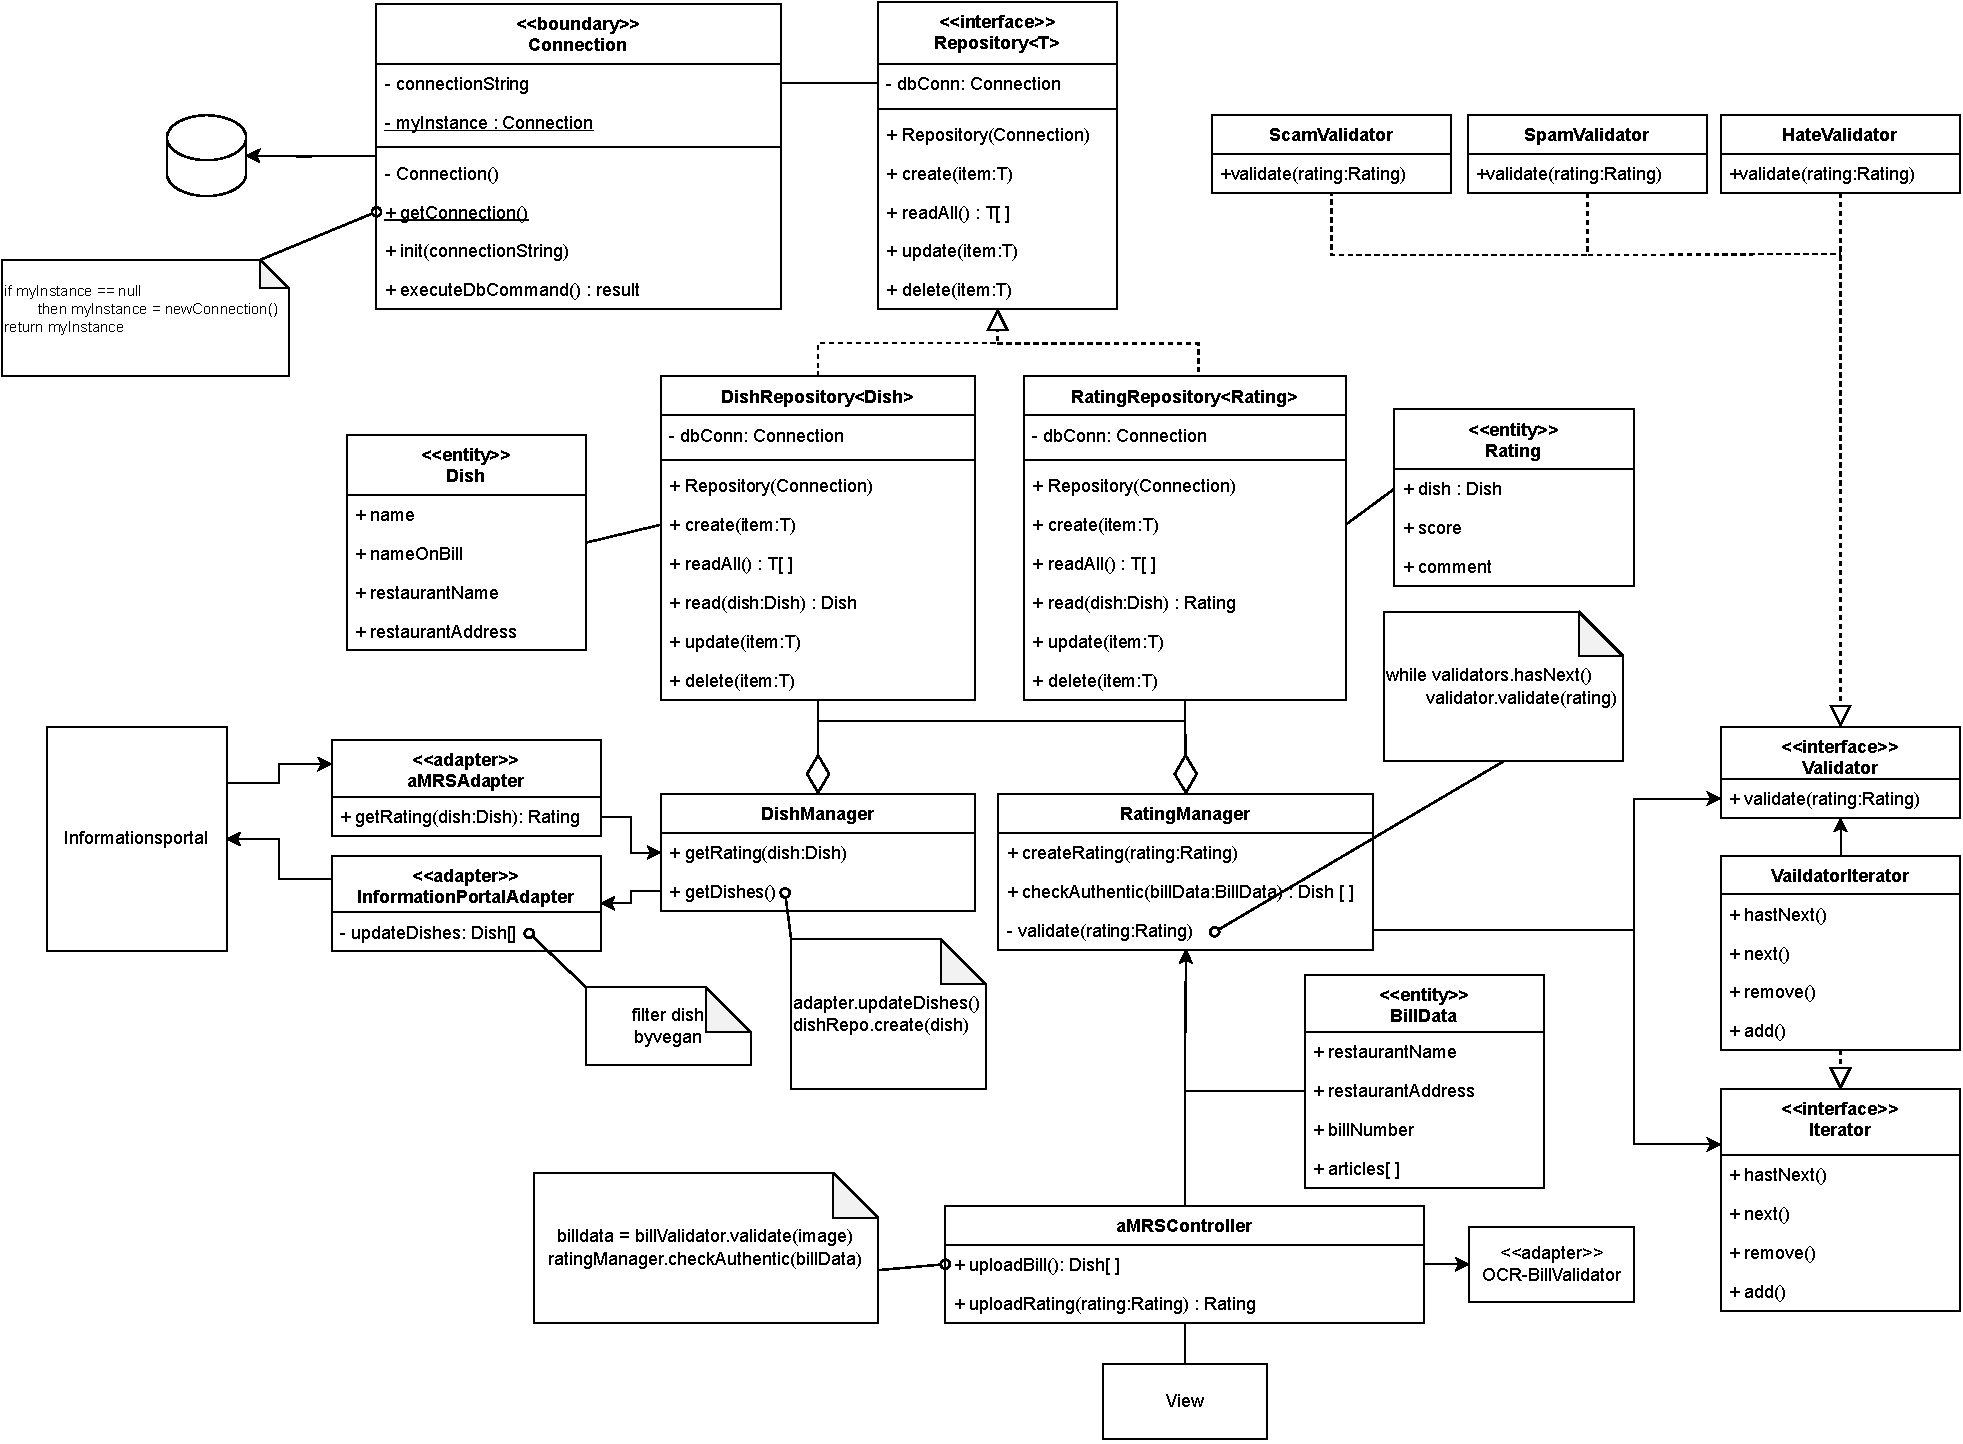
\includegraphics[width=1.3\textwidth,angle=90,keepaspectratio]{images/Fachklassenmodell}
\end{figure}

\section*{Beschreibung der Fachklassen}

\subsection*{Entity}
\textbf{Dish} \\
Die Klasse Dish enthält Informationen über Restaurantname, Restaurantadresse, Rechnungsbezeichner und Gerichtname des
Tagesgerichts.
\newline

\noindent \textbf{BillData} \\
Die Klasse BillData enthält Informationen über Restaurantname, Restaurantadresse, Rechnungsnummer und eine Liste aller
Rechnungsbezeichner der Restaurantrechnung.
\newline

\noindent \textbf{Rating} \\
Die Klasse Rating enthält Informationen über das zu bewertende Dish, eine Wertung und ein Kommentar.

\subsection*{Adapter}
\noindent \textbf{aMRSAdapter}\\
Die Klasse aMRSAdapter gitb dem Informationsportal die Möglichkeit Bewertungen vom \ac{aMRS} abzurufen.
\newline

\noindent \textbf{InformationsPortalAdapter}\\
Die Klasse InformationsPortalAdapter gitb dem \ac{aMRS} die Möglichkeit Tagesgerichte vom Informationsportal abzurufen.
Dabei werden die Tagesgerichte nach Klassifikation gefiltert.
\newline

\noindent \textbf{OCR-BillValidator}\\
Die Klasse OCR-BillValidator stellt die Kommunikation von \ac{aMRS} zum externen OCR-System her.


\subsection*{Boundary}
\noindent \textbf{Connection}\\
Die Klasse Connection empfängt Befehle zur Datenspeicherung beziehungsweise zum Datenzugriff.

\subsection*{Klasse}
\noindent \textbf{DishRepository<Dish>}\\
Die Klasse DishRepository ist für die Speicherung und den Zugriff auf die Daten der Klasse Dish zuständig.
\newline

\noindent \textbf{RatingRepository<Rating>}\\
Die Klasse RatingRepository ist für die Speicherung und den Zugriff auf die Daten der Klasse Rating zuständig.
\newline

\noindent \textbf{DishManager}\\
Die Klasse DishManager enthält die Logik für das Aktualisieren und Speichern neuer Dish-Objekte, sowie zum Abrufen von
vorhandenen Bewertungen.
\newline

\noindent \textbf{RatingManager}\\
Die Klasse RatingManager enthält die Logik für das Speichern und Validieren neuer Rating-Objekte. Zusätzlich wird das
Objekt BillData auf Authentizität überprüft.
\newline

\noindent \textbf{ScamValidator}\\
Die Klasse ScamValidator ist für die Überprüfung auf Scam in Bewertungen zuständig.
\newline

\noindent \textbf{SpamValidator}\\
Die Klasse SpamValidator ist für die Überprüfung auf Spam in Bewertungen zuständig.
\newline

\noindent \textbf{HateValidator}\\
Die Klasse HateValidator ist für die Überprüfung auf Hass in Bewertungen zuständig.
\newline

\noindent \textbf{ValidatorIterator}\\
Die Klasse ValidatorIterator ist für die Iteration über die Validatoren zuständig.
\newline

\noindent \textbf{aMRSController}\\
Die Klasse aMRSController ist für die Kommunikation zwischen View und RatingManager zuständig.
\newline

\noindent \textbf{View}\\
Die Klasse View stellt die GUI dar.
\section{Systemablaufmodell}\label{sec:Systemablaufmodell}
\begin{figure}
  \centering
  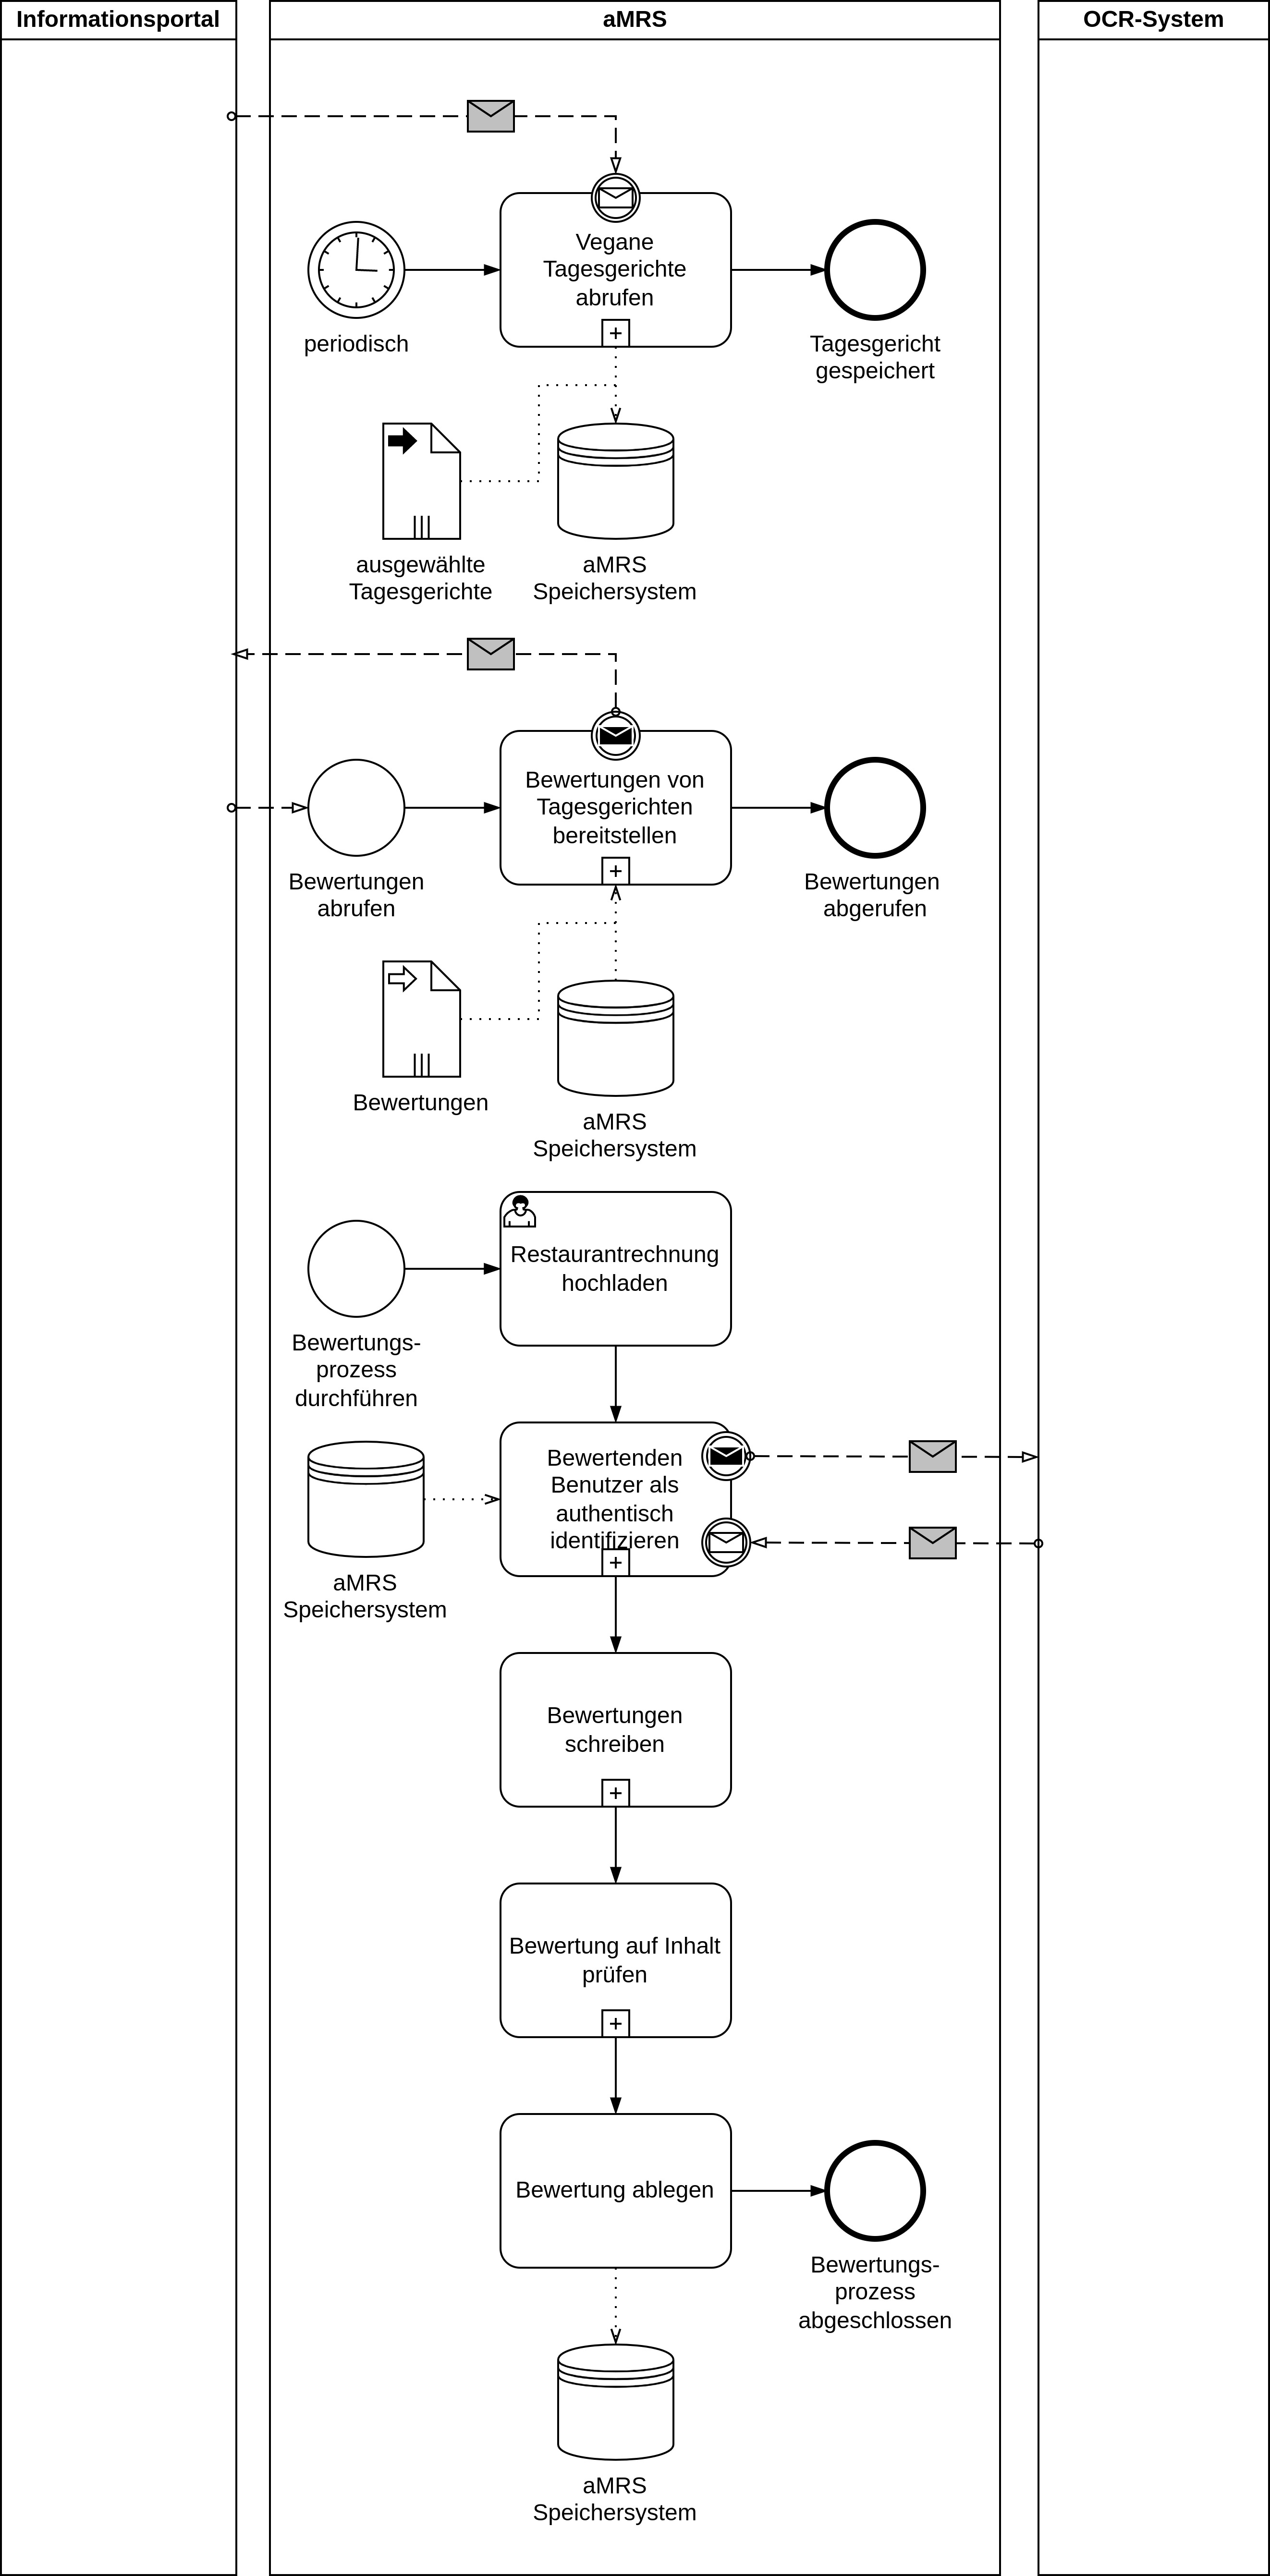
\includegraphics[height=0.8\paperheight]{Systemablaufmodell.jpg}
  \caption{Systemablaufmodell}
  \label{fig:Systemablaufmodell}
\end{figure}
% Ablauf Geschäftsmodelle
% Zusammenspiel der Systeme
% Standardablauf ohne große Abweichungen
Die in Kapitel~\ref{sec:Geschaeftsfaelle} aufgelisteten Geschäftsfälle werden nun in Abbildung~\ref{fig:Systemablaufmodell} zu einem Systemablaufmodell zusammengefügt.
Dabei wird das Zusammenspiel zwischen dem vorhandenen Informationsportal, dem zu entwickelnden System \ac{aMRS} und dem \hyperref[gls:ocr-System]{OCR-System} als externem System dargestellt.

\noindent{}Abbildung~\ref{fig:Systemablaufmodell} zeigt dabei den Standardablauf des Systems und bietet zunächst einen Überblick über die drei Hauptfunktionen des Systems.
In den fünf darauffolgenden Abbildungen (\ref{fig:VeganeTagesgerichteAbrufen}-\ref{fig:BewertungAufInhaltPruefen}) werden die einzelnen Schritte der verschiedenen Geschäftsfälle genauer betrachtet.

\begin{figure}
  \centering
  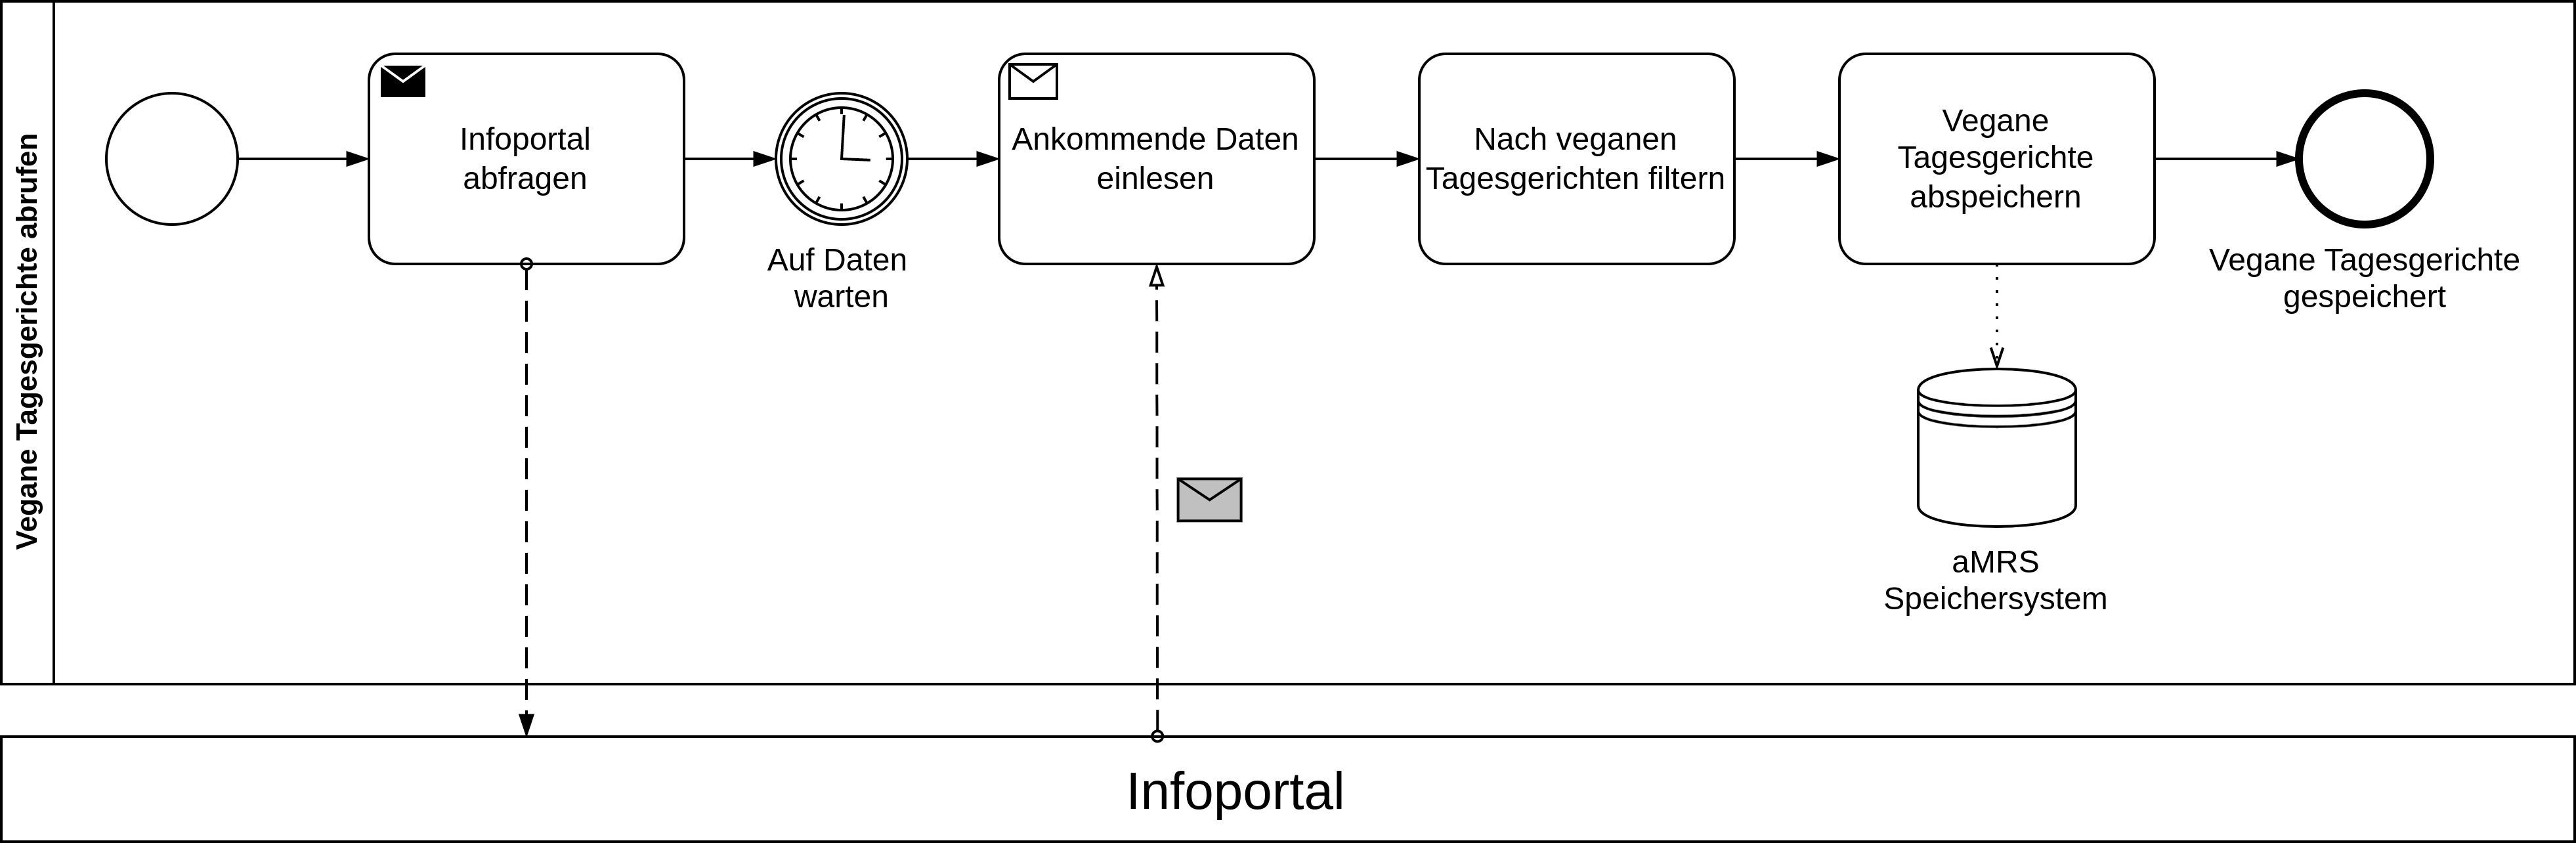
\includegraphics[width=1\linewidth]{VeganeTagesgerichteAbrufen}
  \caption{Systemablaufmodell - Vegane Tagesgerichte abrufen}
  \label{fig:VeganeTagesgerichteAbrufen}
\end{figure}
\begin{figure}
  \centering
  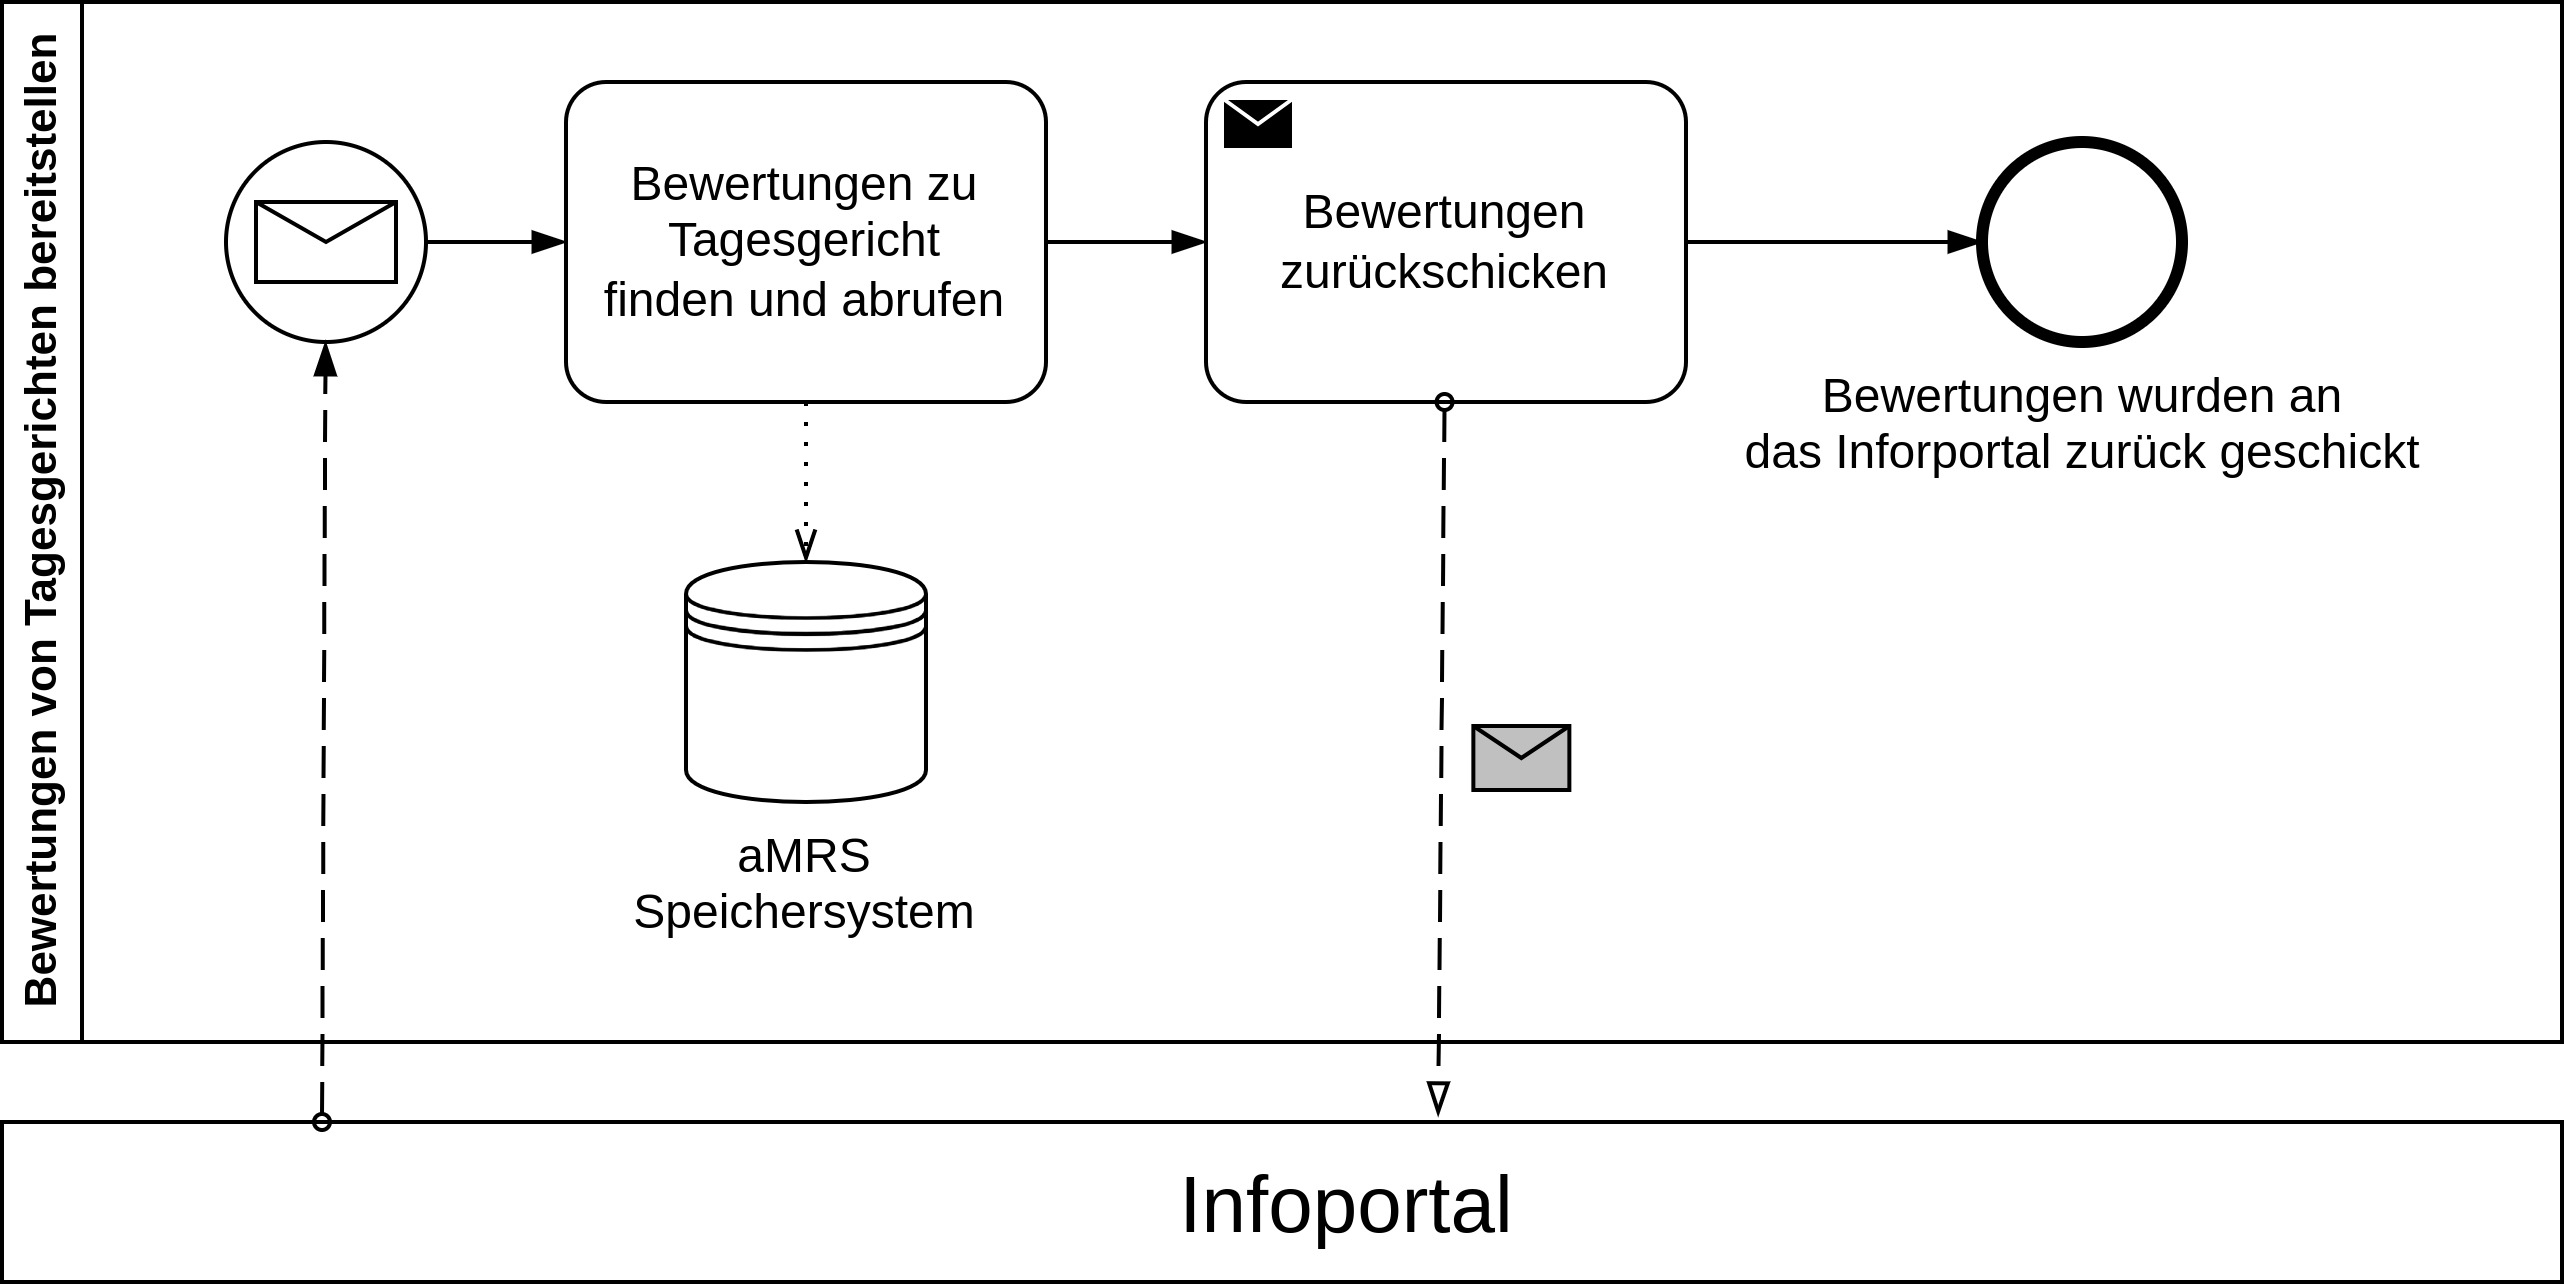
\includegraphics[width=0.8\linewidth]{BewertungenBereitstellen}
  \caption{Systemablaufmodell - Bewertungen von Tagesgerichten bereitstellen}
  \label{fig:BewertungenVonTagesgerichtenBereitstellen}
\end{figure}
\begin{figure}
  \centering
  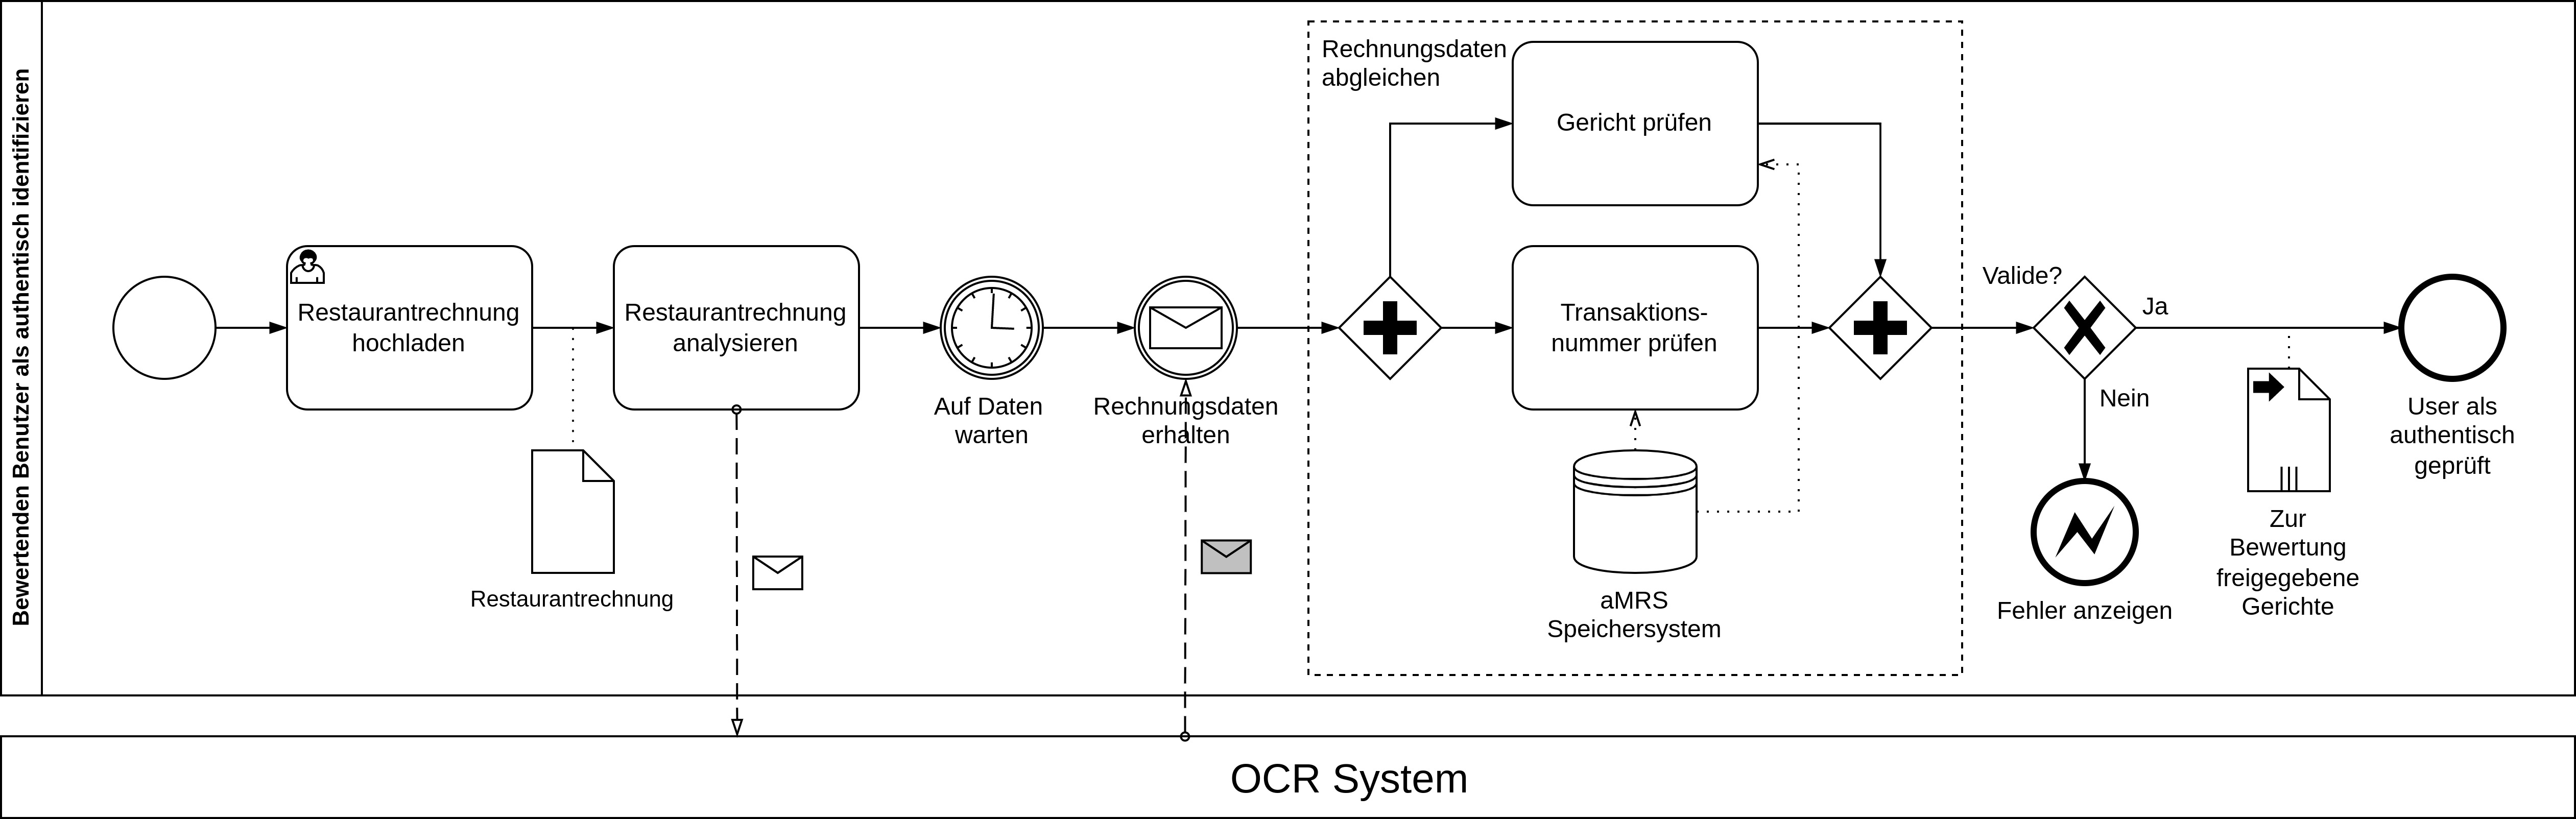
\includegraphics[width=1\linewidth]{BewertendenBenutzerAuthentisch}
  \caption{Systemablaufmodell - Bewertenden Benutzer als authentisch identifizieren}
  \label{fig:BewertendenBenutzerAlsAuthentischIdentifizieren}
\end{figure}
\begin{figure}
  \centering
  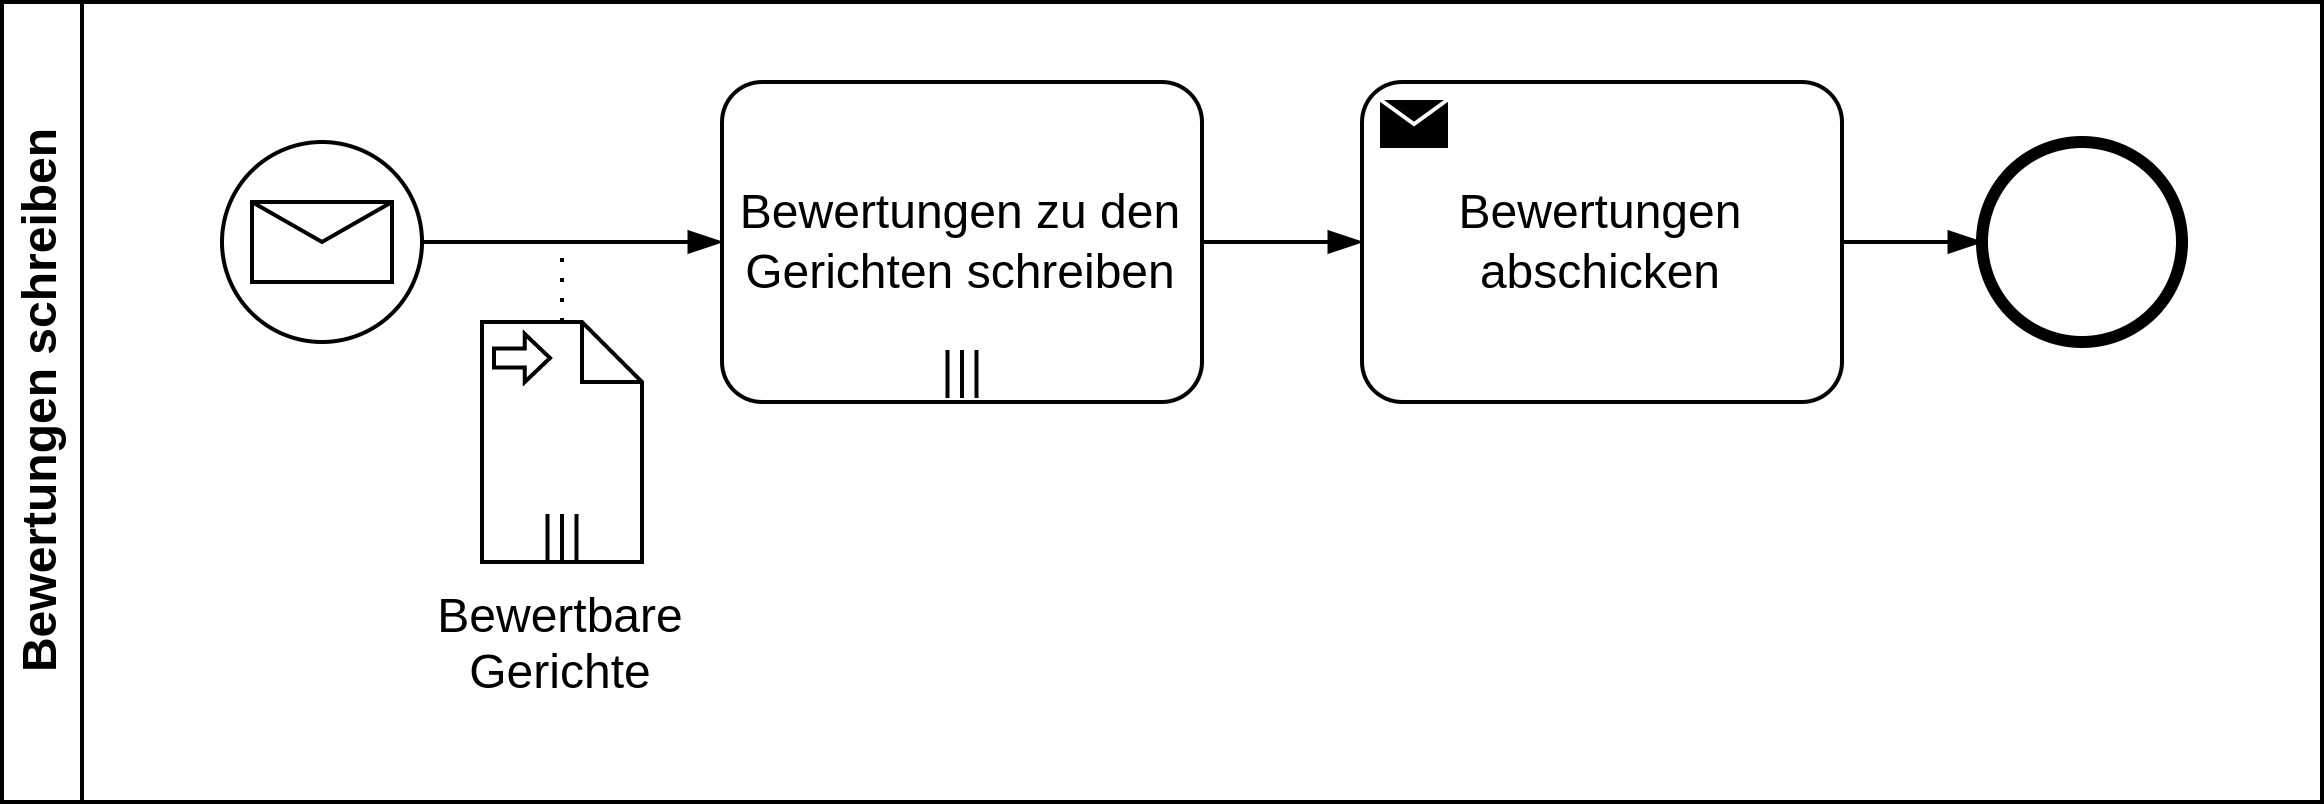
\includegraphics[width=0.9\linewidth]{BewertungSchreiben}
  \caption{Systemablaufmodell - Bewertung schreiben}
  \label{fig:BewertungSchreiben}
\end{figure}
\begin{figure}
  \centering
  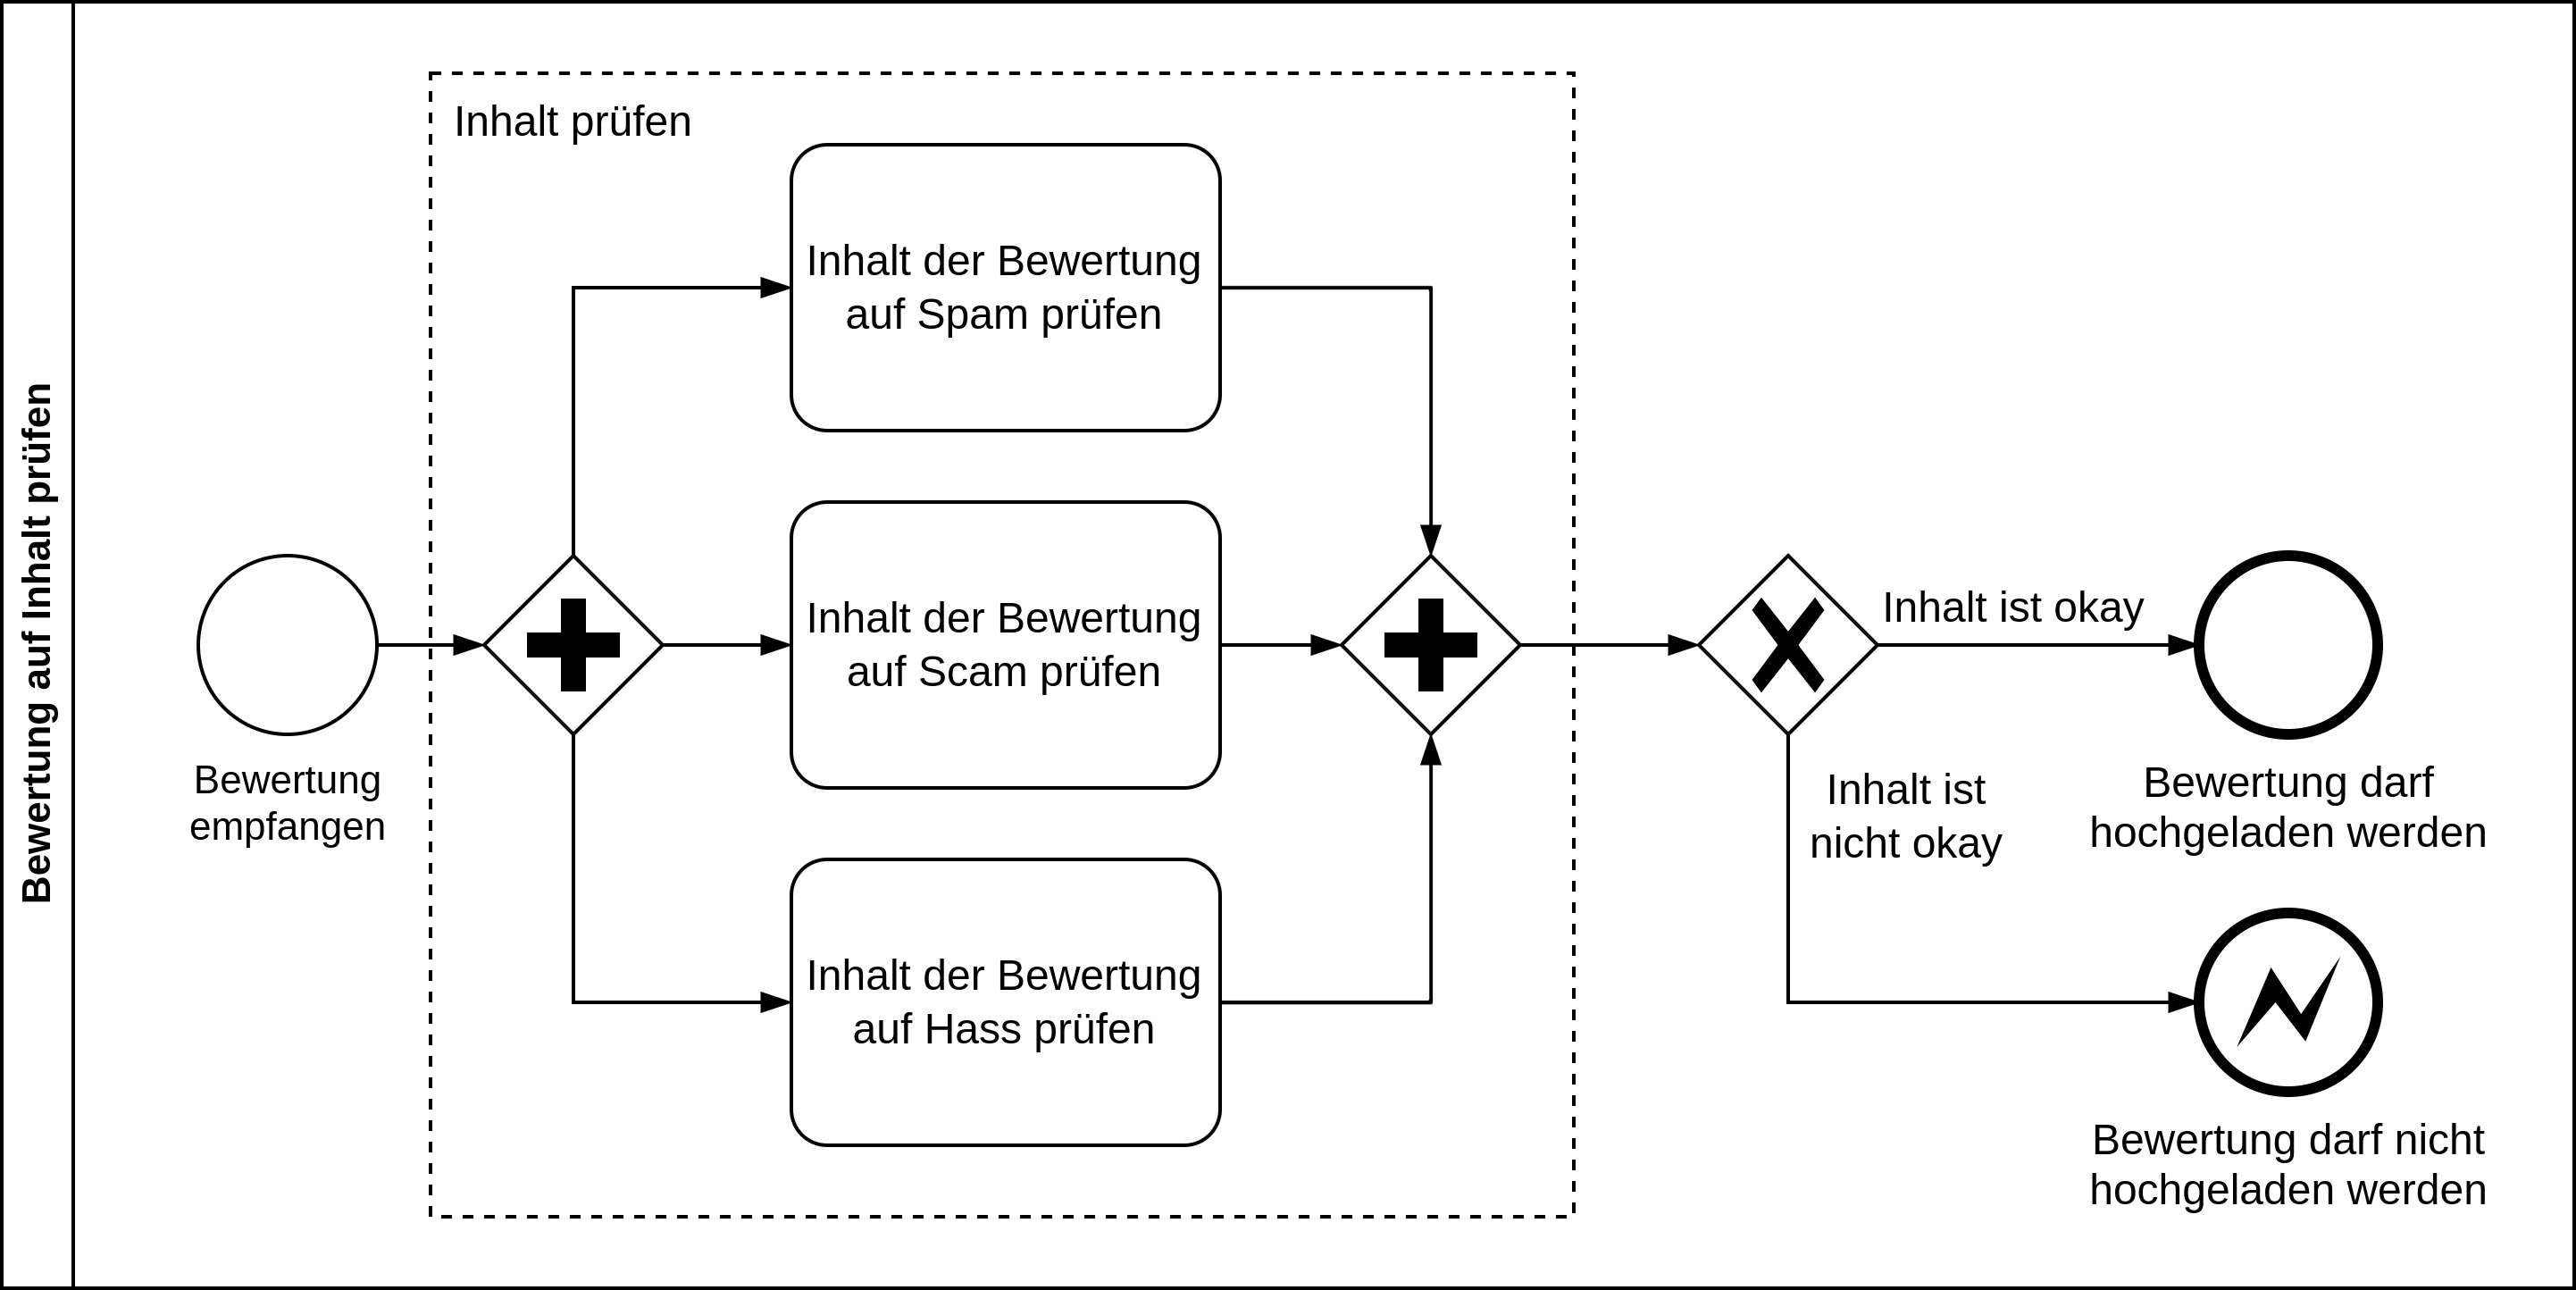
\includegraphics[width=0.9\linewidth]{BewertungInhaltPruefen}
  \caption{Systemablaufmodell - Bewertung auf Inhalt prüfen}
  \label{fig:BewertungAufInhaltPruefen}
\end{figure}

%%%%%%%%%%%%%%%%%%%%%%% Literaturverzeichnis %%%%%%%%%%%%%%%%%%%%%%%
\phantomsection
\addcontentsline{toc}{section}{Literatur}
\printbibliography
\newpage


%%%%%%%%%%%%%%%%%%%%%%%%%%%%%% Anhang %%%%%%%%%%%%%%%%%%%%%%%%%%%%%%
\renewcommand{\thetable}{\Alph{section}.\arabic{table}}
\renewcommand{\thefigure}{\Alph{section}.\arabic{figure}}
\renewcommand{\thelstlisting}{\Alph{section}.\arabic{lstlisting}}
\pagenumbering{Alph}

\begin{appendix}
  \section{Anhang}
\end{appendix}
\end{document}